\documentclass[11pt,a4paper]{article}

\def\nyear {2026}
\def\nterm {Winter}
\def\nlecturer {Danny Neftin}
\def\ncourse {Commutative Algebra}

\makeatletter

% packages
\usepackage{amssymb,amsfonts,amsmath,calc,tikz,pgfplots,geometry,mathtools}
\usepackage{color}   % May be necessary if you want to color links
\usepackage[svgnames]{xcolor}
\usepackage[hidelinks]{hyperref}
\usepackage{forest}
\usepackage{commath} % ew
\usepackage{esvect} % \vv makes vectors
\usepackage{centernot} % for the comparison
\usepackage{esdiff}
\usepackage{esint}
\usepackage{amsthm}
\usepackage{fancyhdr}
\usepackage{bm}
\usepackage{witharrows}
\usepackage{bookmark}
\usepackage{tikz-cd}
\usepackage{quiver}
\usepackage{bbm}
\usepackage{textcomp}
\usepackage{float}
\usepackage{gensymb}
\usepackage{cleveref}
\usepackage{environ}
\usepackage{comment}
\usepackage{cancel}
\usepackage{xparse}

% Inevitable cs
\usepackage{listings}
\usepackage[]{algorithm2e}

% tikz libraries
\usetikzlibrary{positioning}
\usetikzlibrary{matrix}
\usetikzlibrary{arrows}
\usetikzlibrary{bending}
\usetikzlibrary{arrows.meta}
\usetikzlibrary{decorations.markings}
\usetikzlibrary{decorations.pathreplacing}
\usetikzlibrary{decorations.markings}
\usetikzlibrary{patterns}
\usetikzlibrary{backgrounds}

% Page style setup
\pagestyle{fancy}
\fancyhfoffset{0pt}
\renewcommand{\headwidth}{\textwidth}
\geometry{margin=1in}
\pgfplotsset{compat=1.18}
\setlength{\headheight}{14.6pt}
\addtolength{\topmargin}{-1.6pt}
\hypersetup{
    colorlinks=false,
    linktoc=section,
    linkcolor=black,
}

%% maketitle setup
\ifx \nauthor\undefined
  \def\nauthor{Yeheli Fomberg}
\else
\fi

\ifx \nemail\undefined
  \def\nemail{\href{mailto:yp@campus.technion.ac.il}
  {\texttt{<yp@campus.technion.ac.il>}}}
\else
\fi

\ifx \ncoursehead \undefined
  \def\ncoursehead{\ncourse}
\fi

\lhead{\emph{\nouppercase{\leftmark}}}
\ifx \nextra \undefined
  \rhead{
    \ifnum\thepage=1
    \else
      \ncoursehead
    \fi}
\else
  \rhead{
    \ifnum\thepage=1
    \else
      \ncoursehead \ (\nextra)
    \fi}
\fi

\def\notes{notes}
\def\problems{problems}

\ifx \ntype \undefined
  \def\ntype{notes}
\else
\fi

\ifx \ntype \notes
  \let\@real@maketitle\maketitle
  \renewcommand{\maketitle}{\@real@maketitle\begin{center}
  \begin{minipage}[c]{0.9\textwidth}\centering\footnotesize
  These notes are not endorsed by the lecturers.
  I have revised them outside lectures to incorporate supplementary
  explanations, clarifications, and material for fun.
  While I have strived for accuracy, any errors or misinterpretations 
  are most likely mine.
  \end{minipage}\end{center}}
\else
  \ifx \ntype \problems
    \let\@real@maketitle\maketitle
    \renewcommand{\maketitle}{\@real@maketitle\begin{center}
    \begin{minipage}[c]{0.9\textwidth}\centering\footnotesize
    These problems are mostly based on the problem sets I was given
    when taking the course.
    
    While I have strived for accuracy and completeness,
    some of the problems would not have been here without the help of
    friends.
    \end{minipage}\end{center}}
  \else
  \fi
\fi


% theorem environments
\theoremstyle{definition}
\newtheorem{definition}{Definition}[section]
\newtheorem{remark}{Remark}[section]
\newtheorem{example}{Example}[section]
\newtheorem{exercise}{Exercise}[section]
\newtheorem{paradox}{Paradox}[section]
\newtheorem{entry}{Entry}[section]
\newtheorem*{solution}{Solution}
\newtheorem*{question}{Question}
\newtheorem*{answer}{Answer}
\newtheorem*{problem}{Problem}
\theoremstyle{plain}
\newtheorem{theorem}{Theorem}[section]
\newtheorem{proposition}[theorem]{Proposition}
\newtheorem{lemma}[theorem]{Lemma}
\newtheorem{corollary}[theorem]{Corollary}
\newenvironment{proofof}[1]{%
    \renewcommand{\proofname}{Proof of #1}%
    \begin{proof}
}{%
    \end{proof}
}
% tikz customization
\pgfarrowsdeclarecombine{twolatex'}{twolatex'}{latex'}{latex'}{latex'}{latex'}
\tikzset{->/.style = {decoration={markings,
                                  mark=at position 0.999
                                  with {\arrow[scale=2]{latex'}}},
                      postaction={decorate}}}
\tikzset{<-/.style = {decoration={markings,
                                  mark=at position 0.001 with {\arrowreversed[scale=2]{latex'}}},
                      postaction={decorate}}}
\tikzset{-->/.style = {decoration={markings,
                                  mark=at position 0.999
                                  with {\arrow[scale=2]{latex'[sep=0pt -2.5]}}},
                      postaction={decorate}}}
\tikzset{<--/.style = {decoration={markings,
                                  mark=at position 0.001
                                  with {\arrowreversed[scale=2]{latex'[sep=0pt -2.5]}}},
                      postaction={decorate}}}
\tikzset{<->/.style = {decoration={markings,
                                  mark=at position 0.001 with {\arrowreversed[scale=2]{latex'}},
                                  mark=at position 0.999 with {\arrow[scale=2]{latex'}},},
                      postaction={decorate}}}
\tikzset{->-/.style = {decoration={markings,
    mark=at position 0.50+0.225/#1 with {\arrow[scale=2]{latex'}}},
                      postaction={decorate}}}
\tikzset{-<-/.style = {decoration={markings,
                                   mark=at position 0.50-0.225/#1 with {\arrowreversed[scale=2]{latex'}}},
                       postaction={decorate}}}
\tikzset{->>/.style = {decoration={markings,
                                  mark=at position 1 with {\arrow[scale=2]{latex'}}},
                      postaction={decorate}}}
\tikzset{<<-/.style = {decoration={markings,
                                  mark=at position 0 with {\arrowreversed[scale=2]{twolatex'}}},
                      postaction={decorate}}}
\tikzset{<<->>/.style = {decoration={markings,
                                   mark=at position 0 with {\arrowreversed[scale=2]{twolatex'}},
                                   mark=at position 1 with {\arrow[scale=2]{twolatex'}}},
                       postaction={decorate}}}
\tikzset{->>-/.style = {decoration={markings,
                                   mark=at position 0.50+0.450/#1 with {\arrow[scale=2]{twolatex'}}},
                       postaction={decorate}}}
\tikzset{-<<-/.style = {decoration={markings,
                                   mark=at position 0.50-0.450/#1 with {\arrowreversed[scale=2]{twolatex'}}},
                       postaction={decorate}}}

\pgfarrowsdeclare{biggertip}{biggertip}{%
  \setlength{\arrowsize}{1pt}
  \addtolength{\arrowsize}{.1\pgflinewidth}
  \pgfarrowsrightextend{0}
  \pgfarrowsleftextend{-5\arrowsize}
}{%
  \setlength{\arrowsize}{1pt}
  \addtolength{\arrowsize}{.1\pgflinewidth}
  \pgfpathmoveto{\pgfpoint{-5\arrowsize}{4\arrowsize}}
  \pgfpathlineto{\pgfpointorigin}
  \pgfpathlineto{\pgfpoint{-5\arrowsize}{-4\arrowsize}}
  \pgfusepathqstroke
}
\tikzset{
	EdgeStyle/.style = {>=biggertip}
}

\tikzset{circ/.style = {fill, circle, inner sep = 0, minimum size = 3}}
\tikzset{scirc/.style = {fill, circle, inner sep = 0, minimum size = 1.5}}
\tikzset{mstate/.style={circle, draw, black, text=black, minimum width=0.7cm}}

\tikzset{eqpic/.style={baseline={([yshift=-.5ex]current bounding box.center)}}}

\definecolor{mblue}{rgb}{0.2, 0.3, 0.8}
\definecolor{morange}{rgb}{1, 0.5, 0}
\definecolor{mgreen}{rgb}{0, 0.4, 0.2}
\definecolor{mred}{rgb}{0.5, 0, 0}

% topology
\DeclareMathOperator{\dfr}{dfr} % deformation retract
\newcommand{\Cells}{\text{Cells}}
\newcommand{\RP}{\mathbb{RP}}
\newcommand{\CP}{\mathbb{CP}}

% order theory
\newcommand{\join}{\vee}
\newcommand{\meet}{\wedge}

% algebraic geometry
\DeclareMathOperator{\Rad}{Rad} % Radical of modules
\DeclareMathOperator{\Spec}{Spec}
% \renewcommand{\div}{\mathrm{div}} % divisors
\DeclareMathOperator{\Mer}{Mer} % Meromorphic functions
\DeclareMathOperator{\Exc}{Exc} % Exceptional divisor
\DeclareMathOperator{\Td}{Td} % Todd classes

% algebra

\DeclareMathOperator{\trdeg}{tr.deg.}
\DeclareMathOperator{\odd}{odd}
\DeclareMathOperator{\even}{even}
\DeclareMathOperator{\lcm}{lcm}
\DeclareMathOperator{\ord}{ord}
\DeclareMathOperator{\codim}{codim}
\DeclareMathOperator{\Ann}{Ann}
\DeclareMathOperator{\Ext}{Ext}
\DeclareMathOperator{\Sym}{Sym}
\DeclareMathOperator{\Out}{Out}
\DeclareMathOperator{\Aut}{Aut}
\DeclareMathOperator{\End}{End}
\DeclareMathOperator{\Inn}{Inn}
\DeclareMathOperator{\Mat}{Mat}
\DeclareMathOperator{\Fix}{Fix}
\DeclareMathOperator{\std}{std}
\DeclareMathOperator{\sgn}{sgn}
\DeclareMathOperator{\adj}{adj}
\DeclareMathOperator{\id}{id}
\DeclareMathOperator{\op}{op}
\DeclareMathOperator{\tr}{tr}
\DeclareMathOperator{\diag}{diag}
\DeclareMathOperator{\rank}{rank}
\DeclareMathOperator{\rk}{rk}
\DeclareMathOperator{\coker}{coker}
\DeclareMathOperator{\Mult}{Mult} % multiplier algebra
\DeclareMathOperator{\Frac}{Frac} % fraction field
\DeclareMathOperator{\Rat}{Rat}
\DeclareMathOperator{\Gal}{Gal}
\newcommand{\ioplus}{\overset{\text{int}}{\oplus}} % interior direct sum
\newcommand{\GG}{\mathcal G} % Galois correspondence
\newcommand{\FF}{\mathcal F} % Galois correspondence
\newcommand{\cupp}{\smile} % cup product
\newcommand{\capp}{\frown} % cap product
\newcommand{\actson}{\curvearrowright}
\newcommand{\bra}{\left\langle}
\newcommand{\ket}{\right\rangle}
\newcommand{\idealin}{\triangleleft\,}
\newcommand{\normalin}{\triangleleft\,}
\newcommand{\ip}[2]{\left\langle #1, #2 \right\rangle}
\newcommand{\bigslant}[2]
{{\raisebox{.2em}{$#1$}\left/\raisebox{-.2em}{$#2$}\right.}}
\newcommand{\properideal}{%
  \mathrel{\ooalign{$\lneq$\cr\raise.22ex\hbox{$\lhd$}\cr}}}

% categories
\newcommand{\cat}[1]{\mathbf{#1}}
\newcommand{\Ch}{\cat{Ch}} % Chain complexes   
\newcommand{\Set}{\cat{Set}}
\newcommand{\Grp}{\cat{Grp}}
\newcommand{\Ab}{\cat{Ab}}
\newcommand{\Ring}{\cat{Ring}}
\newcommand{\CRing}{\cat{CRing}}
\newcommand{\Top}{\cat{Top}}
\newcommand{\Vect}{\cat{Vect}}
\newcommand{\cmod}{\cat{mod}}

%% matrix groups
\newcommand{\GL}{\mathrm{GL}}
\newcommand{\Or}{\mathrm{O}}
\newcommand{\PGL}{\mathrm{PGL}}
\newcommand{\PSL}{\mathrm{PSL}}
\newcommand{\PSO}{\mathrm{PSO}}
\newcommand{\PSU}{\mathrm{PSU}}
\newcommand{\SL}{\mathrm{SL}}
\newcommand{\msl}{\mathrm{sl}}
\newcommand{\SO}{\mathrm{SO}}
\newcommand{\Spin}{\mathrm{Spin}}
\newcommand{\Sp}{\mathrm{Sp}}
\newcommand{\SU}{\mathrm{SU}}
\newcommand{\U}{\mathrm{U}}
\let\char\relax
\newcommand{\char}{\text{char}}

% analysis
\renewcommand{\Re}{\mathrm{Re}}
\renewcommand{\Im}{\mathrm{Im}}
\NewDocumentCommand{\dx}{o}{
  \IfNoValueTF{#1}
    {\dif x}                  % if no optional argument
    {\dif^{#1} \!x}         % if optional argument
}
\NewDocumentCommand{\dy}{o}{
  \IfNoValueTF{#1}
    {\dif y}                  % if no optional argument
    {\dif^{#1} \!y}         % if optional argument
}
\newcommand{\dt}{\dif t}
\newcommand{\du}{\dif u}
\newcommand{\dv}{\dif v}
\newcommand{\dz}{\dif z}
\newcommand{\ds}{\dif s}
\newcommand{\dw}{\dif w}
\newcommand{\dr}{\dif r}
\newcommand{\dm}{\dif m}
\newcommand{\df}{\dif f}
\newcommand{\dV}{\dif V}
\newcommand{\dS}{\dif S}
\newcommand{\dA}{\dif \mathrm{A}}
\newcommand{\dmu}{\dif \mu}
\newcommand{\dnu}{\dif \nu}
\newcommand{\dtheta}{\dif \theta}
\newcommand{\domega}{\dif \omega}
\newcommand{\dsigma}{\dif \sigma}
\newcommand{\dtau}{\dif \tau}
\newcommand{\dvarphi}{\dif \varphi}
\renewcommand{\dif}{\mathrm{d}}
\renewcommand{\Dif}{\mathrm{D}}
\renewcommand{\triangle}{\Delta}
\newcommand{\ptriangle}{\partial \triangle}
\DeclareMathOperator{\im}{im}
\DeclareMathOperator{\cis}{cis}
\DeclareMathOperator{\rot}{rot}
\DeclareMathOperator{\vspan}{span}
\DeclareMathOperator{\grad}{grad}
\DeclareMathOperator{\curl}{curl}
\DeclareMathOperator{\esssup}{esssup}
\newcommand{\hodge}{{\mathnormal{\star}}}
\DeclareMathOperator{\range}{range}
\DeclareMathOperator{\Hom}{Hom}
\DeclareMathOperator{\Int}{Int}
\DeclareMathOperator{\Conv}{Conv} % convex hull
\newcommand{\ind}{\mathbbm{1}}
\DeclareMathOperator{\Res}{Res}
\DeclareMathOperator{\graph}{graph}
\DeclareMathOperator{\diam}{diam}
\DeclareMathOperator{\supp}{supp}
\DeclareMathOperator{\Vol}{Vol} % Volume
\DeclareMathOperator{\Area}{Area} % Area
\DeclareMathOperator{\area}{area}
\DeclareMathOperator{\Ind}{Ind} % Index
\newcommand{\length}{\mathrm{length}}

% logic
\DeclareMathOperator{\MOD}{MOD}
\DeclareMathOperator{\Theory}{Theory}
\newcommand{\notimplies}{%
  \mathrel{{\ooalign{\hidewidth$\not\phantom{=}$\hidewidth\cr$\implies$}}}}

% nice
\newcommand{\half}{\frac{1}{2}}
\newcommand{\pair}{\del}
\newcommand{\taking}[1]{\xrightarrow{#1}}
\newcommand{\otaking}[1]{\xleftarrow{#1}}
\newcommand{\inv}{^{-1}}
\newcommand{\ot}{\leftarrow}
\newcommand{\ninfty}{-\infty}
\newcommand{\pinfty}{+\infty}
\newcommand{\floor}[1]{\left\lfloor #1 \right\rfloor}
\newcommand{\ceil}[1]{\left\lceil #1 \right\rceil}
\newcommand{\viff}{\Big\Updownarrow} % vertical iff
\newcommand{\bmid}{\,\middle\vert\,} % big mid

% probability
\newcommand{\Prob}{\mathbf{P}}
\renewcommand{\vec}[1]{\boldsymbol{\mathbf{#1}}}
\DeclareMathOperator{\Bin}{Bin}
\DeclareMathOperator{\Geo}{Geo}
\DeclareMathOperator{\Poi}{Poi}
\DeclareMathOperator{\Exp}{Exp}
\DeclareMathOperator{\Var}{Var} % Variance
\DeclareMathOperator{\Cov}{Cov}

% special letters
\newcommand{\N}{\mathbb{N}}
\newcommand{\Z}{\mathbb{Z}}
\newcommand{\Q}{\mathbb{Q}}
\newcommand{\R}{\mathbb{R}}
\newcommand{\C}{\mathbb{C}}
\newcommand{\F}{\mathbb{F}}
\newcommand{\E}{\mathbf{E}}
\newcommand{\D}{\mathbb{D}}
\renewcommand{\H}{\mathbb{H}}
\newcommand{\ps}{\mathcal{P}}
\newcommand{\M}{\mathcal{M}}
\renewcommand{\L}{\mathcal{L}}
\renewcommand{\O}{\mathcal{O}}
\renewcommand{\U}{\mathcal{U}}
\newcommand{\Omicron}{O}
\newcommand{\powerset}{\mathcal{P}}

% text
\newcommand{\st}{\text{ s.t. }}
\newcommand{\tand}{\quad \text{and} \quad}
\newcommand{\tor}{\quad \text{or} \quad}
\newcommand{\stand}{\text{ and }}
\newcommand{\stor}{\text{ or }}
\renewcommand{\tt}[1]{\textnormal{\textbf{(#1).}}} %tt=theorem title GET RID OF

% title format
\title{\textbf{\ncourse}}

\ifx \ntype \notes
  \author{Notes taken by \nauthor\, \nemail \\ Based on lectures by \nlecturer}
  \date{\nterm\ \nyear}
\else
  \ifx \ntype \problems
    \author{These problems were solved by \nauthor \\ \nemail}
  \else
  \fi
\fi

\makeatother

\newcommand{\A}{\mathbb A}
\DeclareMathOperator{\Mor}{Mor}
\DeclareMathOperator{\td}{td}
\newcommand{\ccoprod}{\amalg}
\newcommand{\cprod}{\mathbin{\rotatebox[origin=c]{180}{$\amalg$}}}
\newcommand{\cC}{\mathcal C}
\newcommand{\cD}{\mathcal D}
\newcommand{\ucC}{\underline{\cC}}
\newcommand{\ucD}{\underline{\cD}}

\pgfplotsset{
    myCustomStyle/.style={
        axis lines=middle,
        xlabel={$x_1$},
        ylabel={$x_2$},
        samples=200,
        grid=both,
        width=10cm,
        height=6cm,
        enlargelimits=true,
        legend pos=outer north east
    }
}

% \tikzset{every picture/.style={
%     every path/.style={very thick},
% }}

\begin{document}
\maketitle

% Insert cool image here

\newpage
\tableofcontents
\newpage

\setcounter{section}{-1}
\section{Terminology}

The origin of commutative algebra is found in multiple fields:
\begin{itemize}
  \item Algebraic geometry -- algebraic varieties are usually given
    by rings or a quotient rings of the form $K[x_1,\dots,x_n] / (f_1 \cdots f_n)$.
  \item Algebraic number theory --
    there is a correspondence with rings of the form $\Q[\alpha]$.
\end{itemize}

\begin{remark}[Terminology]
  Some reminders and remarks on terminology:
  \begin{enumerate}
    \item[(1)] Throughout the course all rings are commutative with unity.
    \item[(2)] Recall that a subring is required to have the same unity as its
      parent ring.
    \item[(3)] In order to check if a subset of a ring $R$ is a subring
      it suffices to check closure under multiplication, subtraction,
      and that the unity element is the same.
    \item[(4)] A homomorphism of rings $f \colon R \to S$
      is a map that preserves addition and multiplication,
      and we also require $f(1_R) = 1_S$.
    \item[(5)] A field is a ring $R \neq \set{0}$ in which every nonzero element
      is invertible.
    \item[(6)] An ideal $I \subset R$ is an additive subgroup which is closed
      under multiplication by $R$.
      That is, $R \cdot I \subseteq I$.
    \item[(7)] The ideal generated by elements $a_1,\dots,a_m \in R$ is
      $(a_1,\dots,a_m) := R a_1 + \cdots + R a_m$.
    \item[(8)] The quotient ring  is $R/I := \set{r + I \mid r \in R}$,
      where $r_1 + I = r_2 + I$ if and only if $r_1 - r_2 \in I$.
  \end{enumerate}
\end{remark}

\begin{example}
  Let $R$ be a ring, and let $x_1,\dots,x_n$ be variables.
  A polynomial a formal expression of the form:
  \[
    \sum_{i_1,\dots,i_n \geq 0}
      a_{i_1 \dots i_n} x_1^{i_1} x_2^{i_2} \cdots x_n^{i_n},
  \]
  such that $a_{i_1 \dots i_n} \in R$ are zero except for finitely many indices.
\end{example}

\begin{example}
  Note that polynomials may be equivalent as functions,
  but different as formal expressions.
  For example in $R = \Z/2\Z$
  we have the equivalency $x^2 + x \equiv 0$,
  but it is clear that these two polynomials
  are different as formal expressions.
\end{example}

\newpage
\section{Introduction through geometry}

\begin{definition}[Affine variety]
  Let $k$ be a field.
  The affine $n$-space $\A^n_k$ is the set
  \[
    \A^n_k := \set{(x_1 \dots x_n) \mid x_i \in k \st \forall i=1,\dots,n}.
  \]
  For a set of polynomials $S \subseteq k[x_1,\dots,x_n]$ we define
  its set of zeros (also called zero locus) as:
  \[
    V(S) := \set{x \in \A^n \mid f(x) = 0 \quad \forall f \in S},
  \]
  This set is called the affine (algebraic) variety associated with $S$.
\end{definition}

\begin{remark}
  The symbol $\A$ stands for the word ``Affine'' since this space
  closely resembeles the notion of an affine space in the theory of vector
  spaces.
\end{remark}

\begin{remark}
  If $S = (f_1,\dots,f_n)$ is a finite set,
  we sometimes will write $V(S) = V(\set{f_1,\dots,f_n})$ as $V(f_1,\dots,f_n)$.
\end{remark}

\begin{example}
  Let $k = \R$, and $S = \set{x_1^2 + x_2^2 - 1}$.
  Then $V(S) = S^1$.
  \begin{center}
    \begin{tikzpicture}
      \draw[very thick] (90:1) arc[start angle=90, end angle=-270, radius=1];
      \draw[-->] (-3, 0) -- (3, 0) node[right] {$x_1$};
      \draw[-->] (0,-1.5) -- (0,1.8) node[right] {$x_2$};
    \end{tikzpicture}
  \end{center}
  If $S = \set{x_1 x_2}$ then $V(S)$ is simply the axes themselves:
  \begin{center}
    \begin{tikzpicture}
      \draw[very thick] (-3, 0) -- (3, 0) node[right] {};
      \draw[very thick] (0,-1.5) -- (0,1.8) node[right] {};
      \draw[-->] (-3, 0) -- (3, 0) node[right] {$x_1$};
      \draw[-->] (0,-1.5) -- (0,1.8) node[right] {$x_2$};
    \end{tikzpicture}
  \end{center}
  If $S = \set{x_1 x_2 - 1}$ then $V(S)$ is the graph of the function
  $x_1 \mapsto 1/x_1$,
  and if $S = \set{x_1^2 + x_2^2 + 1}$ then $V(S)$ is the empty set.
\end{example}

\begin{remark}
  A nonexample of an affine variety is $V(\sin x)$,
  since $\sin x$ is not a polynomial.
  Even though we will not discuss nonaffine varieties in this course,
  there is still a significant number of mathematicians working
  with many such abstract objects
  including: projective varieties, schemes, o minimal structures.
\end{remark}

\begin{definition}[Ideal map]
  Let $X \subseteq \A_k^n$ be an affine variety.
  We define a map that sends
  ideals to varieties $I \colon \set{\text{Varieties}} \to \set{\text{Ideals}}$
  as follows:
  \[
    I(X) := \set{f \in k[x_1,\dots,x_n] \mid f(x) = 0 \quad \forall x \in X}.
  \]
  We sometimes call the ideal $I(X)$ simply ``the ideal of $X$''.
\end{definition}

\begin{remark}
  The ideal map $I \colon \set{\text{Varieties}} \to \set{\text{Ideals}}$
  clearly has an inverse relation with the map
  $V \colon \set{\text{Sets of polynomials}} \to \set{\text{Varieties}}$.
  They are the inverse maps of each other
  in some sense which we will discuss soon.
\end{remark}

\begin{remark}[Coordinate ring]
  Let $X \subseteq \A_k^n$ be an affine variety.
  We define the coordinate ring (or ring of algebraic functions on $X$),
  to be the quotient $k[X] := k[x_1,\dots,x_n] / I(X)$.
\end{remark}

\begin{remark}
  Recall that $p_1,p_2 \in k[x_1,\dots,x_n]$ define the same function
  if and only if $p_1 - p_2 \equiv 0$ or equivalently $p_1 - p_2 \in I(X)$,
  or equivalently $p_1 + I(X) = p_2 + I(X)$.
  This implies that $k[X] := k[x_1,\dots,x_n] / I(X)$ is a ring of functions
  (not formal expressions).
  In fact, the motivation for the coordinate ring (ring of functions)
  is exactly this property.
  The intuitive way to think about $k[X]$ is as the ring of functions
  (that or polynomial) of the form $f \colon X \to k$.
  This intuition would be useful throught this section.
\end{remark}

\begin{example}
  Let $a = (a_1,\dots,a_n) \in \A_k^n$.
  Is it a variety?
  Yes!
  since $\set{a} = V(x_1 - a_1,x_2 - a_2,\dots,x_n - a_n)$.
  Note that this also happens to be the intersection of all the axes
  $\bigcap V(x_i - a_i)$.
\end{example}

\begin{proposition}
  \label{prop:point-ideal}
  Let $a \in \A_k^n$.
  Then $I := I(\set{a}) = (x_1 - a_1,x_2 - a_2,\dots,x_n - a_n) := M_a$,
  where $(x_1 - a_1,x_2 - a_2,\dots,x_n - a_n)$ is the ideal generated
  by $x_1 - a_1,x_2 - a_2,\dots,x_n - a_n$.
\end{proposition}
\begin{proof}
  We will show this by double sided containment.
  It is clear that $M_a \subset I$.

  For the other direction,
  consider the substitution map $\pi_a \colon k[x_1,\dots,k_m] \to k$
  given by $g \mapsto g(a)$.
  Since $M_a \subseteq \ker \pi_a$
  we get a surjection $k[x_1,\dots,x_n]/M_a \to k[x_1,\dots,x_n]/\ker \pi_a$,
  given by $g + M_a \mapsto g + \ker \pi \mapsto g(a)$,
  and since $\pi_a$ is a surjection the first isomorphism theorem
  gives $k[x_1,\dots,x_n]/\ker \pi_a \cong k$.

  The homomorphism (surjection) is one-to-one since
  \[
    p(x_1,\dots,x_n) = p(a_1,\dots,a_n) \pmod{M_a}
  \]
  (we can transfer them to constants by substituion $x_i = a_i$)
  for all $p \in k[x_1,\dots,x_n]$, so it follows that the map is injective,
  thus $M_a$ is maximal,
  and $\bar \pi$ is an isomorphism and $\ker \pi_a = I(a)$.
\end{proof}

\begin{remark}
  We can see that the coordinate ring $k[x_1,\dots,x_n]/I(X)$
  gives us a correspondence between algebraic varieties (algebraic geometry)
  and quotient rings (commutative algebra).
  In particular, by \Cref{prop:point-ideal} we saw that
  $I(a)$ are maximal, and thus $k[x_1,\dots,x_n]/I(a)$ are fields.
\end{remark}

\begin{definition}[Subvarieties]
  Let $X \subseteq \A^n_k$ be a variety.
  Then for a set of polynomials in the coordinate ring $S \subseteq k[X]$,
  we say that $V(S) = V_X(S) := \set{x \in X \mid f(x) = 0\quad \forall f \in S}$
  is a subvariety of $X$.
\end{definition}

\begin{remark}
  It is clear that sets of the form $V_X(Y)$ are exactly the varieties in $\A_k^n$
  contained in $X$.
  This is why they are called the subvarieties of $X$.
\end{remark}

\begin{question}
  Which objects in commutative algebra
  have a correspondence with the subvarieties of $X$?
\end{question}

\begin{definition}[Subideal map]
  Let $X \subseteq \A^n$ be a variety.
  For a subset $Y \subset X$ we define
  \[
    I(Y) = I_X(Y) := \set{f \in k[X] \mid f(y) = 0 \quad \forall y \in Y}.
  \]
  We call $I_X(Y)$ ``the ideal of $Y$ (in $X$)''.
\end{definition}

\begin{remark}
  \label{rmk:varieties-containment}
  Every variety is a subvariety.
  Also note that $S \subset S'$ implies $V(S) \supseteq V(S')$,
  and that $Y \subset Y'$ implies $I(Y) \supseteq I(Y')$.
\end{remark}

\begin{lemma}
  \label{lem:quotient-rings}
  Let $X$ be a variety and $k[X]$ its ring of functions.
  If $Y \subseteq X$ is a subvariety then $k[Y] \cong k[X]/I(Y)$.
  Moreover, $Y = V(I(Y))$.
\end{lemma}
\begin{proof}
  Consider the map restriction map $r \colon k[X] \to k[Y]$
  given by $f + I(X) \mapsto f + I(Y)$.
  It is a ring homomorphism whose kernel is $I(Y)$,
  and therefore the first isomorphism theorem completes the first part of the
  proof.

  For the second part, by definition we have $Y \subseteq V(I(Y))$.
  Since $Y$ is a subvariety, we get that $Y = V(S)$ for some $S \subset k[X]$.
  In particular $I(Y) = I(V(S))$ and by definition $I(Y) = I(V(S)) \supseteq S$.
  Now by applying $V$ on both sides and using \Cref{rmk:varieties-containment},
  we can conclude that $V(I(Y)) \subseteq V(S)$, which completes the proof.
\end{proof}

\begin{remark}
  By \Cref{lem:quotient-rings}
  it follows that subvarieties correspond to quotient rings.
\end{remark}

\begin{question}
  Which objects in commutative algebra
  have a correspondence with morphisms of subvarieties?
\end{question}

\begin{exercise}
  Let $Y = V(y_2 - y_1^2) \subseteq \A_{\R}^2$.
    \begin{center}
  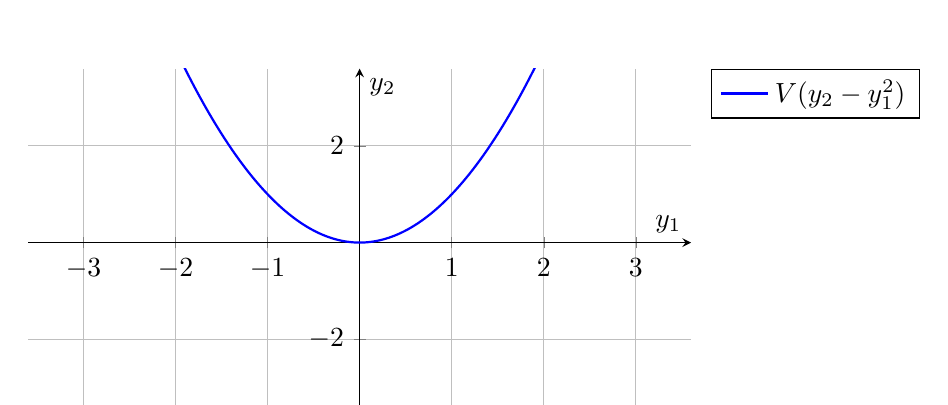
\begin{tikzpicture}
    \begin{axis}[myCustomStyle,
        xmin=-3, xmax=3,
        ymin=-3, ymax=3,
        xlabel={$y_1$},
        ylabel={$y_2$},
        domain=-3:3]
      \addplot[blue, thick] {x^2};
      \addlegendentry{$V(y_2 - y_1^2)$}
    \end{axis}
  \end{tikzpicture}
    \end{center}
  We know that $I(Y) = (y_2 - y_1^2)$.
  Show that $K[Y] \cong K[y_1,y_2]/(y_2 - y_1^2) \cong k[y_1]$.
  This isomorphism of rings shows that the parabola curve
  is homeomorphic to the $x$-axis.
\end{exercise}

\begin{definition}[Morphism of varieties]
  Let $X \subseteq \A_k^n$ and $Y \subseteq \A_k^m$ be varieties.
  A map $f \colon X \to Y$ is called a morphism if there exist
  $f_1,\dots,f_m \in k[x_1,\dots,x_n]$ such that $f(x) = (f_1(x),\dots,f_m(x)) \in Y$
  for every $x \in X$.
\end{definition}

\begin{definition}[Induced homomorphism]
  A morphism $f$ induces a homomorphism on the coordinate rings
  $f^* \colon k[Y] \to k[X]$ by $g + I(Y) \mapsto g \circ f + I(X)$.
  This map is well defined since $X \taking{f} Y \taking{g} k$.
\end{definition}

\begin{example}
  Let $X = \A_{\R}^1$ and $Y = V(y_2 - y_1^2) \subseteq \A_{\R}^2$.
  The coordinate ring $\R[X]$ is simply $\R[x_1]$
  and $\R[Y] = \R[y_1,y_2] / (y_2 - y_1^2)$.

  Then the map $f \colon X \to Y$ given by $x \mapsto (x,x^2)$
  is a morphism inducing $f^* \colon \R[Y] \to \R[X]$
  by $g \mapsto g \circ f \colon x \mapsto g(x,x^2)$.
\end{example}

\begin{remark}
  We can summarize the connections we have seen so far between geometry and
  algbera in the following table:
  \begin{center}
    \begin{tabular}{c|c}
    Geometry                        & Algebra        \\ \hline
    Variety $X$          & The function algebra $k[X]$ \\
    Subvariety $Y$ of $X$   & Ideal $I(Y) \idealin k[X]$ of functions on $X$ vanishing on $Y$         \\
    Morphism $f \colon X \to Y$ of varieties & Ring homomorphism $f^* \colon k[Y] \to k[X]$.     
    \end{tabular}
  \end{center}
\end{remark}
% Lecture 2

\begin{remark}[Galois connection]
  \label{rmk:galois-connection}
  Recall that there is a correspondence between algebraic varieties
  and subsets of polynomials.
  \[
  \begin{tikzcd}
    \set{X \subseteq \A_k^n}
    \arrow[r, shift left, "I"] &
    \set{S \subseteq k[x_1,\dots,x_n]}
    \arrow[l, shift left, "V"],
  \end{tikzcd}
  \]
  where $V \colon S \mapsto \set{x \mid p(x) = 0 \quad \forall p \in S}$
  and $I \colon X \mapsto \set{p \mid p(x) = 0 \quad \forall x \in X}$.
\end{remark}

\begin{remark}
  We will call an ideal in the image of $I$ is a \textit{geometric ideal}.
  This is a temporary name until we understand these type of ideals better.
\end{remark}

\begin{definition}[Galois connection]
  Let $C,D$ be partially ordered sets
  and let $V \colon C \to D$ and $I \colon D \to C$ be maps.
  The ordered pair $(V,I)$ is called a Galois connection if $X \le Y$
  implies $I(X) \geq I(Y)$ and $V(I(X)) \geq X$,
  and similarly $S \le T$ implies $V(S) \geq V(T)$ and $I(V(S)) \geq S$.
\end{definition}

\begin{remark}
  The correspondence in \Cref{rmk:galois-connection} is a galois connection
  with the partial order of containment.
\end{remark}

\begin{exercise}
  \label{ex:galois-correspondence}
  Suppose that $(V,I)$ is a Galois connection.
  Show that:
  \begin{enumerate}
    \item[(1)] If $X \in \im V$ then $V(I(X)) = X$.
    \item[(2)] Similarly, if $J \in \im I$ then $I(V(J)) = J$.
  \end{enumerate}
\end{exercise}

\begin{corollary}
  There is a one-to-one (invertible) correspondence:
  \[
  \begin{tikzcd}
    \set{X \subseteq \A_k^n \text{ subvariety}}
    \arrow[r, shift left, "I"] &
    \set{\text{Geometric ideals } I \normalin k[x_1,\dots,x_n]}
    \arrow[l, shift left, "V"],
  \end{tikzcd}
  \]
\end{corollary}
\begin{proof}
  Directly from \Cref{ex:galois-correspondence} since we have seen
  that this is a Galois connection.
\end{proof}

\begin{corollary}
  For $X \subseteq \A_k^n$ we have that $V(I(X))$ is the smallest
  subvariety containing $X$ (this is a type of closure operation with
  respect to being a subvariety).
  Similarly, for a subset $S \subseteq k[x_1,\dots,x_n]$
  we get that $I(V(S))$ is the smallest geometric ideal containing $S$.
\end{corollary}
\begin{proof}
  Let $X \subseteq Y \subseteq \A_k^n$ be a subvariety of $\A_k^n$
  containing $X$.
  Define $Z := V(I(X))$ and
  replace $Y$ by $Y \cap Z$ to obtain that $X \subseteq Y \subseteq Z$.
  This implies that $I(X) \supseteq I(Y) \supseteq I(Z)$,
  and then $Z := V(I(X)) \subseteq V(I(Y)) \subseteq V(I(Z)) = Z$
  and since $Y$ is a subvariety $V(I(Y)) = Y$,
  and hence $Y = Z$.

  Similarly,
  we can let $I(V(S)) = \overline S$ (closure with respect to geometric ideals)
  and carry out the proof in the same manner.
\end{proof}

\begin{remark}
  The subvarieties of $\A_k^n$ are the closed subsets in a topology closed
  the Zarisky topology. (We will show this later)
\end{remark}

\begin{remark}
  The closure of a set $X \subseteq \A_k^n$
  in the Zariski topology is $\overline X := V(I(X))$.
\end{remark}

\begin{question}
  What are the geometric ideals?
\end{question}

\begin{example}[Nongeometric ideal]
  Let $R := k[x]$ for some field $k$ (recall that $k[x]$ is a PID).
  We know that for any irreducible $f \in k[x]$,
  the ideal $(f)$ is maximal.
  Note that $(x^2) \subsetneq (x) \normalin k[x]$
  but $V(x^2) = V(x) = \set{0}$.
  Since we have seen that there is a one-to-one correspondence of geometric
  ideals and subvarieties, either $(x)$ or $(x^2)$ is a nongeometric ideal.
  Since we have
  \[
    I(V(x^2)) = I(\set{0}) = (x),
  \]
  we get that $(x^2)$ isn't geometric.
\end{example}

\begin{remark}
  We have seen that points are subvarities,
  so by the Galois connection,
  intuitively, they must correpond to maximal ideals.
\end{remark}

\begin{remark}[Point ideals]
  For every point $a \in \A_k^n$
  we have defined the evaluation map $\pi_a \colon k[x_1,\dots,k_n] \to k$
  with $f \mapsto f(a)$,
  which has kernel $M_a = (x_1 - a_1,\dots, x_n - a_n)$.
  We notice that $M_a$ is indeed a maximal ideal,
  and it is associated with the point $a$.

  An ideal of the form $M_a = (x_1 - a_1,\dots, x_n - a_n)$
  is called a \textit{point ideal}.
\end{remark}

\begin{question}
  Is every maximal ideal a point ideal?
\end{question}
\begin{answer}
  Not always.
  For example, the ideal $(x^2 + 1) \normalin \R[x]$ is maximal,
  but it is not a point ideal.
\end{answer}

\begin{lemma}
  Let $k$ be a field.
  Then every maximal ideal in $k[x]$ is a point ideal if and only if
  $k = \overline k$ ($k$ is algebraically closed).
\end{lemma}
\begin{proof}
  Since $k[x]$ is a PID, its maximal ideals are generated by an irreducible
  polynomial $f \in k[x]$.
   But now all irreducible polynomials are of degree $1$ if and only
   if $k$ is algebraically closed,
   which completes the proof (the ideal is a point ideal).
\end{proof}

\begin{theorem}[Weak nullstellensatz]
  \label{thm:weak-null}
  If $k$ is an algebraically closed field,
  then every maximal ideal in $k[x_1,\dots,x_n]$ is a point ideal.
\end{theorem}

\begin{corollary}
  If $k$ is an algebraically closed field and $X \subseteq \A_k^n$
  is a variety,
  then every maximal ideal in $k[X] := k[x_1,\dots,x_n] / I(X)$
  is a point ideal $(\overline{x_1 - a_1},\dots,\overline{x_n - a_n})$
  where $\overline{x_1 - a_1} = x_1 - a_1 + I(X)$.
\end{corollary}
\begin{proof}
  Follows from the weak nullstellensatz theorem and the correspondence theorem:
  \[
  \begin{tikzcd}
    \set{\text{Ideals } J \normalin k[x_1,\dots,x_n] \text{ containing } I}
    \arrow[r, shift left,] &
    \set{\text{Ideals in } k[x_1,\dots,x_n] / I(X)}
    \arrow[l, shift left,],
  \end{tikzcd}
  \]
\end{proof}

% closed points

% Hilbert nullstellensatz

\begin{question}
  What are the geometric ideals?
\end{question}

\begin{definition}[Radical of an ideal]
  Let $I \normalin R$ be an ideal.
  Then we define the radical of the ideal to be:
  \[
    \sqrt{I} := \set{f \in R \mid f^n \in I \text{ for some } n \in \N}.
  \]
\end{definition}

\begin{remark}
  \label{rmk:geometric-are-radical}
  Suppose $I = I(X)$ is a geometric ideal.
  Then if $f^n \in I$, we get $f^n(x) = 0$ for all $x \in X$,
  so $f(x) = 0$ for all $x \in X$, which implies that $f \in I$.
  This means that any geometric ideal is necessarily radical.
\end{remark}

\begin{definition}[Radical ideal]
  A radical $I \normalin R$ is said to be a radical ideal if $\sqrt I = I$.
\end{definition}

\begin{example}
  Consider the example $(x^2 + 1) \normalin \R[x]$.
  It is a maximal ideal, but it is not a geometric ideal.
  This may seem as a contradiction to Hilbert's nullstellensatz theorem,
  but it is not because the field $\R$ is not algebraically closed.
\end{example}

\begin{theorem}[Hilbert's nullstellensatz, strong form, 1893]
  Let $k = \overline k$ be an algebraically closed field.
  Then $I$ is geometric if and only if $I$ is radical.
  In other words, we have the correpondence:
  \[
  \begin{tikzcd}
    \set{X \subseteq \A_k^n \text{ subvariety}}
    \arrow[r, shift left, "I"] &
    \set{\text{Radical ideals } I \normalin k[x_1,\dots,x_n]}
    \arrow[l, shift left, "V"],
  \end{tikzcd}
  \]
\end{theorem}
\begin{lemma}
  The weak version of Hilbert's nullstellensatz implies its strong version.
\end{lemma}
\begin{proof}
  We know from \Cref{rmk:geometric-are-radical} that all geometric ideals
  are radical.

  On the other direction, let $I = \sqrt{I}$ be a radical ideal,
  and write $I = (f_1,\dots,f_m)$.
  Assume that for every $f \in I(V(I))$
  we have $f^l \in I$.
  Becuase $I = \sqrt{I}$, it follows from the claim
  that for every $f \in I(V(I))$ we have $f \in I$.
  It follows that $I(V(I)) \subseteq I$,
  and since from the Galois connection the opposite containment always
  holds we get that $I(V(I)) = I$, and therefore $I$ is geometric.
  We now proceed to prove the assumption.

  By Rabinowitsch's trick (\Cref{prop:rabinowitsch-trick}), there exist $g_0,\dots,g_m \in k[x_0,\dots,x_n]$
  such that $1 = g_0 f_0 + \cdots + g_m f_m$.
  Next, substitute the expression $x_0 = \frac{1}{f(x_1,\dots,x_n)}$.
  This is a substitution homomorphism
  from $k[x_0,\dots,x_n]$
  to the fraction field $k[x_1,\dots,x_n] = \Frac(k[x_1,\dots,x_n])$.
  Then
  \[
    1 = \underbrace{g_0 (1 - 1)}_{=\,0} +
    \sum_{i=1}^{m} g_i\del{\frac{1}{f},x_1,\dots,x_n} f_i(x_1,\dots,x_n).
  \]
  By clearing the denominators we get:
  \[
    f^l =
    \sum_{i=1}^{m} h_i f_i \in I
  \]
  for some $l \in \N$.
\end{proof}

\begin{proposition}[Rabinowitsch trick, 1929]
  \label{prop:rabinowitsch-trick}
  Consider $f,f_1,\dots,f_m \in k[x_1,\dots,x_n]$ as polynomials in the extended
  ring $k[x_0,x_1,\dots,x_n]$,
  denote $I = (f_1,\dots,f_m)$, and suppose that $f$
  vanishes whenever $f_1,\dots,f_m$ vanish.
  Then for $f_0 = 1 - x_0 f$, we have
  \[
    (f_0,f_1,\dots,f_m) = k[x_0,\dots,x_n].
  \]
\end{proposition}
\begin{proof}
  Assume, by way of contradiction,
  that $(f_0,\dots,f_m)$ is contained in some maximal ideal $M$.
  By \Cref{thm:weak-null} we get that $M = I(a)$ for some point $a \in V(I)$.
  However, since $f \in I(V(I))$ and $a \in V(I)$ we get that $f(a) = 0$,
  and then $f_0(a) = 1$,
  which is a contradiction to $f_0 \in I(a)$.
\end{proof}

\begin{remark}
  Intuitively,
  adding $x_0$ is like adding $1/f$ to the ring.
  This process is what we will later call ``localization''.
\end{remark}

\begin{question}
  Why can we assume that $I = (f_1,\dots,f_m)$ is finitely generated?
\end{question}
\begin{solution}
  Hilbert's basis theorem.
\end{solution}

\begin{theorem}[Hilbert's basis theorem, 1890]
  Every ideal $I \idealin k[x_1,\dots,x_n]$ is finitely generated.
  More generally, every increasing chain $I_1 \subseteq I_2 \subseteq \cdots $
  of ideals stabilizes.
  Equivalently, $k[x_1,\dots,x_n]$ is Noetherian.
\end{theorem}

\begin{proofof}{\Cref{thm:weak-null}, unfinished}
  Let $M \idealin k[x_1,\dots,x_n]$ be a maximal ideal.
  Observe that $a \in V(M)$ if and only if $I(a) = M$.

  Since $M$ is maximal, the quotient $k[x_1,\dots,x_n] / M$ is a field.
  We also have another field $k \subset k[x_1,\dots,x_n]$.
  Note that $k \cong k[x_1,\dots,x_n] / M$ implies that
  $x_i + M = a_i + M$ for some $a_i \in k$ and thus $x_i - a_i \in M$
  for all $i$, and therefore $M = I((a_1,\dots,a_n))$.
  We have that $k \hookrightarrow k[x_1,\dots,x_n] / M$ by sending
  $a \mapsto a + M$.

  % need to show that every field $F$ that is finitely generated
  % as a ring over $k$ is a finite field extension of $k$.
\end{proofof}

\begin{remark}
  Let $R$ be a ring.
  If $I \normalin R$ is an ideal then:
  \begin{enumerate}
    \item[(1)] $I$ is maximal if and only if $R/I$ is a field.
    \item[(2)] $I$ is prime if and only if $R/I$ is an integral domain.
    \item[(3)] $I$ is radical if and only if $R/I$ is reduced (has no nilpotent elements).
  \end{enumerate}
  In particular we have the implications:
  \[
    I \text{ maximal} \implies
    I \text{ prime} \implies
    I \text{ radical}
  \]
\end{remark}

\begin{question}
  We saw that maximal ideals correspond to points.
  What do prime ideals correspond to geometrically?
\end{question}
\begin{example}
  Let $X = V(x_1 \cdot x_2) \subseteq \A^2$.
  We get that:
  \[
    \begin{tikzpicture}[eqpic]
      \draw[very thick] (-2, 0) -- (2, 0) node[right] {};
      \draw[very thick] (0,-1.5) -- (0,1.8) node[right] {};
    \end{tikzpicture} \quad \raisebox{-0.25cm}{=} \qquad
    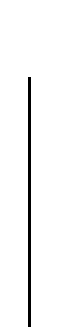
\begin{tikzpicture}[eqpic]
      \draw[very thick] (0,-1.5) -- (0,1.8) node[right] {};
    \end{tikzpicture} \quad \raisebox{-0.25cm}{+} \quad
    \raisebox{-0.25cm}{
    \begin{tikzpicture}[eqpic]
      \draw[very thick] (-2, 0) -- (2, 0) node[right] {};
  \end{tikzpicture}}
  \]
  In some sense $X$ is reducible since we can decompose it into the
  sum of two varieties.
  Note that the ideal $(x_1 \cdot x_2) \idealin \R[x_1,x_2]$ is not a prime
  ideal.
\end{example}

\begin{definition}[Reducible subvariety]
  Let $Y \subseteq X$ be a subvariety.
  Then $Y$ is called reducible if and only if there exists two subvarieties
  $\emptyset \neq Y_1,Y_2 \subsetneq Y$ such that $Y = Y_1 \cup Y_2$.
  If $Y$ is not reducible, it is called an irreducible subvariety.
\end{definition}


\begin{lemma}
  We have that $Y \subseteq X$ is irreducible if and only if $I_X(Y)$
  is prime.
\end{lemma}
\begin{proof}
  Note that $I_X(Y)$ is non-prime if and only if there exist
  $f_1,f_2 \in k[X] \setminus I_X(Y)$ such that $f_1 f_2 \in I_X(Y)$,
  and this happens if and only if there exists varieties
  $Y_1 = V_Y(f_1)$ and $Y_2 = V_Y(f_2)$,
  and by definition $\emptyset \neq Y_1,Y_2 \subsetneq Y$
  and $Y_1 \cup Y_2 = V_Y(f_1 \cdot f_2) = Y$,
  which is if and only if $Y$ is reducible (tricky),
  which completes the lemma.
\end{proof}

\begin{remark}
  Note that by definition we always
  have that $V_Y(f_1 \cdot f_2) = V(f_1) \cup V(f_2)$.
  Think what this means geometrically.
\end{remark}

\begin{exercise}
  Is $V(x^2 + y^2) \subseteq \A^2$ reducible?
\end{exercise}
\begin{solution}
  The answer depends on $\A$.
  Remember the charatarization of irreducible subvarieties
  by prime ideals.
  It is now easy to conclude that $V(x^2 + y^2)$ is irreducible over $\R$,
  but reducible over $\C$ by $x^2 + y^2 = (x + iy)(x - iy)$.
\end{solution}

\begin{remark}[Zariski topology]
  We have the following connections between varieties and ideals:
  \begin{center}
\begin{tabular}{c|c}
Algebra                        & Geometry        \\ \hline
$V(J) \supseteq V(I)$          & $J \subseteq I$ \\
$V(I + J) = V(I) \cap V(J)$    & $I + J$         \\
$V(I \cap J) = V(I) \cup V(J)$ & $I \cap J$     
\end{tabular}
  \end{center}
  Note that we even have $V(\sum_{j \in J} I_j) = \bigcap_{j \in J} V(I_j)$
  when $J$ is infinite.
  However, the last property only holds for finite intersections.
  This means that $V(I)$ satisfy the basic properties of ``closed sets'',
  and indeed, the topology generated by declaring the varieties as closed
  sets is a topology, and it is called the \textit{Zariski topology}.
\end{remark}

\begin{remark}
  Recall that for a set of ideals $\set{I_{\alpha}}_{\alpha \in A}$
  we define:
  \[
    \sum_{\alpha \in A} I_{\alpha} =
    \set{\sum_{\alpha \in A} i_{\alpha} \,\middle\vert\,
      i_k = 0 \text{ for all but finitely many } \alpha \in A}.
  \]
\end{remark}

\begin{proposition}
  \label{prop:zariski-topology}
  Let $I,J,I_{\alpha} \normalin k[X]$
  where $\alpha \in A$.
  Then:
  \begin{enumerate}
    \item[(1)] $\bigcap_{\alpha \in A} V(I_{\alpha}) = V(\sum_{\alpha \in A} I_{\alpha})$
    \item[(2)] $V(I) \cup V(J) = V(I \cap J)$.
  \end{enumerate}
  As a consequence, the Zariski topology is a topology.
\end{proposition}

\begin{exercise}
  Deduce that $\sum_{\alpha \in A} I_{\alpha}$
  is the smallest ideal that contains $\set{I_{\alpha}}_{\alpha \in A}$.
\end{exercise}

\begin{lemma}
  \label{lem:zariski-topology}
  We have that $\sqrt{I} \cap \sqrt{J} = \sqrt{I \cap J} = \sqrt{I \cdot J}$.
\end{lemma}

\begin{proofof}{\Cref{prop:zariski-topology}}
  By the fact $V(I) = V(\sqrt{I})$ for any ideal $I$
  (since the radical of the ideal has the same set of zeros)
  we get that $V(I \cap J) = V(\sqrt{I \cap J})$.
  Then from \Cref{lem:zariski-topology} we conclude that:
  \[
    V(I \cap J) = V(\sqrt{I \cap J}) = V(\sqrt{I \cdot J}) = V(I \cdot J) =
    \set{x \mid f(x)g(x) = 0 \quad \forall f \in I \stand g \in J}.
  \]
  where $I \cdot J = (f \cdot g \mid f \in I \stand g \in J)$.
  Thus, from simple set theoretic arguments we have:
  \[
    V(I \cap J) =
    \set{x \mid f(x) = 0 \stor g(x) = 0 \quad \forall f \in I \stand g \in J} =
    V(I) \cup V(J).
  \]
  The proof for the infinite case and the zero locus of an intersection of ideals
  is left as an exercise.
\end{proofof}

% closed points
% to come: \sqrt{I} = \bigcap_{P prime & I \subseteq P} P

\newpage

\section{Categories and modules}
\subsection{Cateogries and functors}

\begin{definition}[Small cateogry]
  A (small) category $\cC$ consists of:
  \begin{enumerate}
    \item[(1)] A class $\ucC$ whose elements are called
      the objects of $\mathcal C$,
    \item[(2)] For every $A,B \in \ucC$
      we have a set of morphisms $\Mor_{\cC}(A,B)$ whose elements are called
      morphisms from $A$ to $B$.
    \item[(3)] For every $A \in \ucC$ we require a distinguished element
      $1_A \in \Mor_{\mathcal C}(A,A)$.
    \item[(4)] For every $A,B,C \in \ucC$,
      a map $\Mor(B,C) \times \Mor(A,B) \to \Mor(A,C)$
      \[
        (f,g) \mapsto f \circ g
      \]
      subject to the conditions:
      \begin{enumerate}
        \item[(a)] $1_B \circ f = f = f \circ 1_A$ for every $A,B \in \ucC$
          and every $f \in \Mor(A,B)$.
        \item[(b)] $(f \circ g) \circ h = f \circ (g \circ h)$ for every
          $A,B,C,D \in \ucC$
          and every $h \in \Mor(A,B)$, $g \in \Mor(B,C)$, and $f \in \Mor(C,D)$.
      \end{enumerate}
  \end{enumerate}
\end{definition}

\begin{remark}
  When we are talking about a specific category,
  for example the category of $\Set$ (which we will soon discuss),
  we sometimes abuse notation and write $A \in \Set$ instead of
  $A \in \underline{\Set}$, and we also write $\Set(A,B) := \Mor_{\Set}(A,B)$.
\end{remark}

\begin{example}
  The category $\Set$ is a category whose objects are sets,
  and for all sets $A,B,C \in \Set$ we have:
  \begin{enumerate}
    \item[(1)] $\Set(A,B)$ are the functions from $A$ to $B$.
    \item[(2)] $1_A$ is the identity map.
    \item[(3)] The map $\Set(B,C) \times \Set(A,B) \to \Set(A,C)$ is composition
      of functions
  \end{enumerate}
\end{example}

\begin{remark}
  Similarly, we can define the categories $\Grp$, $\CRing$ and $\Ab$
  which are the categories of groups, commutative rings, and abelian groups respectively.
\end{remark}

\begin{example}
  Topological spaces and continuous maps
  form a category called $\Top$.
  We denote the cateogry of pointed topological spaces by $\Top_*$.
\end{example}

\begin{example}
  Algebraic sets over $k$ form a category $_k \Set$
  while regular maps are morphisms.
\end{example}

\begin{example}
  Every cateogry $\mathcal C$ has an opposite cateogry which we denote
  by $\mathcal C^{\op}$ which we define by ``reversing arrows''.
  That is, $\ucC^{\op} := \ucC$ and $\Mor_{\cC^{\op}}(A,B) := \Mor_{\cC}(B,A)$.
\end{example}

\begin{remark}
  Morphisms need not be maps between sets.
  For example, every poset $(X,\le)$ defines a cateogry $\mathcal C$
  whose objects are the elements of $X$ and for every $A,B \in \mathcal C$
  we define:
  \[
    \Mor(A,B) :=
    \begin{cases}
      \set{f_{AB}} &A \le B, \\
      \emptyset &\text{otherwise}.
    \end{cases}
  \]
\end{remark}

\begin{definition}[Covariant functor]
  Let $\mathcal C$ and $\mathcal D$ be cateogries.
  A (covariant) functor $F \colon \mathcal C \to \mathcal D$ consists of:
  \begin{enumerate}
    \item[(1)] A map
      $\underline F \colon \underline{\mathcal C} \to \underline {\mathcal D}$
      denoted $C \mapsto F(C)$.
    \item[(2)] For every $A,B \in \ucC$ a map
      $F_{A,B} \colon \Mor_{\mathcal C}(A,B) \to \Mor_{\mathcal D}(F(A),F(B))$
      denoted $f \mapsto F(f)$ such that
      \begin{enumerate}
        \item[(a)] $F(1_A) = 1_{F(A)}$.
        \item[(b)] $F(f \circ g) = F(f) \circ F(g)$.
      \end{enumerate}
  \end{enumerate}
\end{definition}

\begin{remark}
  In slightly less formal words,
  a covariant functor is a function between cateogries that preserves
  their structure, or simply, a ``homomorphim of categories''.
\end{remark}

\begin{definition}[Contravariant functor]
  A contravariant functor $F \colon \mathcal C \to \mathcal D$
  is a covariant functor from $\mathcal C^{\op} \to \mathcal D$.
\end{definition}

\begin{remark}
  Note that a functor $F \colon \cC \to \cD$ such that
  for every $f \in \Mor(A,A')$ and $g \in \Mor(A',A'')$ satisfies
  $F(f \circ g) = F(g) \circ F(f)$ is still a contravariant functor.
\end{remark}

\begin{remark}
  Small categories and functors between them constitute a cateogry.
\end{remark}

\begin{example}[Forgetful functor]
  The forgetful functor is a functor $F \colon \Grp \to \Set$
  sending all groups their underlying sets,
  and preserving morphisms.
\end{example}

\begin{example}
  The map $\pi_1 \colon \Top_* \to \Grp$ that sends
  a pointed topological space to its fundamental group
  is a functor.
\end{example}

\begin{example}
  The functor $F \colon \Vect_k \to \Vect_k$ sends a vector space $V$
  to its double-dual space $V^{**}$,
  and now we need to find a way to sends a map $f \colon V \to W$
  to a map $f^{**} \colon V^{**} \to W^{**}$.
  Note that if $\lambda \in W^*$ then
  $f^*(\lambda) := \lambda \circ f \in V^*$.
  Now given $\psi \in V^{**}$ we define $f^{**}(\psi) \in W^{**}$ by
  (for every $\lambda \in W^*$) $f^{**}(\psi)(\lambda) := \psi(f^*(\lambda))$.
\end{example}

\begin{example}[Representable functor]
  Every object $A \in \ucC$ defines a functor
  into the cateogry of sets $\Mor(A, -) \colon \mathcal E \to \Set$
  called the functor represented by $A$.
  Since all families of morphisms $\Mor_{\cC}(A,B)$
  are sets, the functor maps any $B \in \ucC$ to $\Mor_{\cC}(A,B) \in \Set$.

  We now have to think how to send an arrow from $B \taking{f} B'$
  to an arrow in the category of sets.
  That is, we need to sends an arrow $B \taking{f} B'$ to a function
  $\Mor_{\cC}(A,B) \to \Mor_{\cC}(A,B')$, and we can do this by
  function composition.
  More precisely, the mapping is $f \mapsto f \circ$,
  where $f \circ \colon \Mor_{\cC}(A,B) \to \Mor_{\cC}(A,B')$
  is the map $(f \circ)(h) = f \circ h \in \Mor_{\cC}(A,B')$.
 
  We also have the contravariant functor $\mathcal C \to \Set$
  denoted $\Mor(-,A) \colon \mathcal C \to \Set$
  which sends $B$ to $\Mor(B,A)$ and $f$ to $\circ f$.
\end{example}
\begin{remark}
  The map $f \circ$ is sometimes denoted $f_*$ and is called the
  pushforward map, while the map $\circ f$ is denote $f^*$ and is called the
  pullback map.
\end{remark}

\begin{definition}[Isomorphism]
  A morphism $A \taking{f} B$ in a cateogry $\cC$ is called an isomorphism
  if there exists $B \taking{g} A$ such that $g \circ f = 1_A$ and
  $f \circ g = 1_B$.
\end{definition}

\begin{definition}[Product]
  A product of two objects $A,B \in \underline{\mathcal C}$ is an object $A \cprod B$
  together with two morphisms $A \otaking{P_A} A \cprod B \taking{P_B} B$
  such that for every object $C$ and all morphisms $A \otaking{Q_A} C \taking{Q_B} B$
  there exists a unique map $\tau \colon C \to A \cprod B$
  such that the following diagram is commutative:
  \[\begin{tikzcd}[ampersand replacement=\&,cramped]
    \&\& {C} \\
    \\
    A \&\& {A \cprod B} \&\& B
    \arrow["{Q_A}"', from=1-3, to=3-1]
    \arrow["{\exists ! \tau}"', dashed, from=1-3, to=3-3]
    \arrow["{Q_B}", from=1-3, to=3-5]
    \arrow["{P_A}"', from=3-3, to=3-1]
    \arrow["{P_B}", from=3-3, to=3-5]
  \end{tikzcd}\]
\end{definition}

\begin{exercise}
  If $(C,P_A,P_B)$, $(D,Q_A,Q_B)$ are products of $A$
  and $B$ then there exists a unique isomorphism $\tau \colon C \to D$
  such that the following diagram commutes:
  \[\begin{tikzcd}[ampersand replacement=\&,cramped]
    \&\& C \\
    \\
    A \&\& D \&\& B
    \arrow["{P_A}"', from=1-3, to=3-1]
    \arrow["{\exists ! \tau}"', dashed, from=1-3, to=3-3]
    \arrow["{P_B}", from=1-3, to=3-5]
    \arrow["{Q_A}"', from=3-3, to=3-1]
    \arrow["{Q_B}", from=3-3, to=3-5]
  \end{tikzcd}\]
\end{exercise}

\begin{definition}[Coproduct]
  A coproduct of $A$ and $B$ is a triple $(A \ccoprod B, i_A, i_B)$
  where $i_A$ and $i_B$ are maps to $A \ccoprod B$ such that for any object $C$
  and all maps $j_A \colon A \to C$ and $j_B \colon B \to C$
  there exists a unique map $f \colon A \ccoprod B \to C$ such that
  the following diagram commutes:
  \[\begin{tikzcd}[ampersand replacement=\&,cramped]
    A \&\& {A \ccoprod B} \&\& B \\
    \\
    \&\& C
    \arrow["{i_A}", from=1-1, to=1-3]
    \arrow["{j_A}"', from=1-1, to=3-3]
    \arrow["{\exists ! f}"', dashed, from=1-3, to=3-3]
    \arrow["{i_B}"', from=1-5, to=1-3]
    \arrow["{j_B}", from=1-5, to=3-3]
  \end{tikzcd}\]
\end{definition}
\begin{remark}
  The coproduct is also uniuqe up to isomorphism.
\end{remark}
\begin{remark}
  Note that the coproduct is defined exactly like we defined product,
  except we reversed the arrows.
  This is a common theme in category theory,
  and pretty much everything we define, we can define in the same
  way but also reverse the arrows.
\end{remark}

\begin{remark}[Existence of products and coproducts]
  Products an coproducts do not always exist.
\end{remark}

\begin{example}
  The following table shows what are the products an coproducts
  in $\Set$, $\Grp$, and $\Ab$.
  \begin{center}
    \begin{tabular}{c|c|c}
    Category & Product        & Coproduct    \\ \hline
    $\Set$   & $\times$       & $\sqcup$     \\
    $\Grp$   & direct product & free product \\
    $\Ab$    & direct product & direct sum   \\
    \end{tabular}
  \end{center}
\end{example}

\subsection{Modules}
The goal of this subsection is to introduce the category of modules.

\begin{definition}[$R$-module]
  An $R$-module is an abelian group $M$ with an action
  $R \times M \to M$ written $(r,m) \mapsto r \cdot m$
  such that for every $r,s \in R$ and $m,n \in M$:
  \begin{enumerate}
    \item[(1)] $1 \cdot m = m$.
    \item[(2)] $r \cdot (s \cdot m) = (rs) \cdot m$.
    \item[(3)] $(r + s) \cdot m = r \cdot m + s \cdot m$ and
      $r \cdot (m + n) = r \cdot m + r \cdot n$.
  \end{enumerate}
\end{definition}

\begin{remark}
  A submodule $N \leqslant M$ is an abelian subgroup preserved by the action
  of $R$.
\end{remark}

\begin{remark}
  In particular $M/N$ is an abelian group with an $R$-module structure.
  That is, the multiplication $r \cdot (m + N) = r \cdot m + N$
  is well defined.
\end{remark}

\begin{example}
  If $R = k$ is a field, then an $R$-module $M$ is a $k$-vector field.
\end{example}

\begin{example}
  If $A$ is an abelian group,
  it as a $\Z$-module structure under the action $\Z \times A \to A$
  defined by $(n,a) \mapsto n \cdot a$,
  where multiplication is just repetitive addition for $\Z_{\geq 0}$,
  and similarly for $\Z_{< 0}$ execpt we multiply by $-1$.
\end{example}

\begin{example}
  Every ideal $I \idealin R$ is an $R$-module.
  It is a submodule of $R$ as an $R$-module.

  Similarly, every submodule of $R$ corresponds to an ideal.
\end{example}

\begin{remark}
  Recall that a group action $G \actson S$ defines
  a homomorphism $\varphi \colon G \to \Sym(S)$
  which we write as $\varphi \colon g \mapsto \varphi_g \in \Sym(S)$
  such that $\varphi_g(s) = g \cdot s$.

  Similarly, for every $R$-module $M$,
  we get a homomorphism $\varphi \colon R \to \End(M)$,
  which is given by $\varphi \colon r \mapsto \varphi_r \in \End(M)$
  defined by $\varphi_r \colon m \mapsto r \cdot m$.
\end{remark}

\begin{remark}
  The objects in the category of $R$-modules are obviously modules.
  The arrows in the category are $R$-modules homomorphisms.
\end{remark}

\begin{definition}[Module homomorphism]
  Let $M,N$ be $R$-modules.
  A map $f \colon M \to N$ is called a homomorphism of $R$-modules
  if it is a homomorphism of abelian groups which preserves the action
  $f(r \cdot m) = r \cdot f(m)$.
\end{definition}

\begin{remark}
  % Cref?
  Homomorphism of an $R$-module for $R$ which is a field
  are linear transformation.
  Homomorphism of an $R$-module for $R = \Z$
  are homomorphisms of abelian groups.
  % what about ideal?
\end{remark}

\begin{remark}
  The cateogry of modules is denoted $R$-$\cmod$.
  The cateogry of right modules is sometimes denoted $\cmod$-$R$.
\end{remark}

\begin{remark}
  For a commutative ring $R$,
  a left $R$-module defines a right $R$-module.
\end{remark}

\begin{remark}
  In fact, $\Hom_{R\text{-}\cmod}(M,N)$ is an $R$-module by:
  \[
    (f + g)(m) := f(m) + g(m) \tand
    (r \cdot f)(m) = f(r \cdot m) = r \cdot f(m).
  \]
\end{remark}

\begin{remark}
  Let $N$ and $M$ be $R$-modules,
  and let $f \colon N \to M$ be a homomorphisms.
  Then $\im(f)$ and $\ker(f)$ are submodules,
  and we define $\coker(f) := N/\im(f)$.
\end{remark}

\begin{remark}
  We have that $\Hom_{R\text{-}\cmod}(M,N)$ is an $R$-module by:
  \[
    (f + g)(m) := f(m) + g(m) \tand
    (r \cdot f)(m) = f(r \cdot m) = r \cdot f(m).
  \]
\end{remark}

\begin{remark}
  The isomorphism theorems from group theory also work similarly
  for modules.
\end{remark}

\begin{definition}[Universal property of the kernel]
  Let $f \colon M \to N$ be a module homomorphism.
  Then $\ker f$ makes the following diagram commute:
  \[\begin{tikzcd}[ampersand replacement=\&,cramped]
    M \&\& N \\
    \\
    {\ker (f)}
    \arrow["f", from=1-1, to=1-3]
    \arrow["i", from=3-1, to=1-1]
    \arrow["0"', from=3-1, to=1-3]
  \end{tikzcd}\]
  The universal property of the kernel,
  is that for any other object $K$ in the cateogry of $R$-modules
  that makes the previous diagram commute,
  there exists a unique $\varphi \colon K \to \ker(f)$
  such that the following diagram commute:
  \[\begin{tikzcd}[ampersand replacement=\&,cramped]
    \& M \&\& N \\
    \\
    \& {\ker (f)} \\
    K \\
    \arrow["f", from=1-2, to=1-4]
    \arrow["i", from=3-2, to=1-2]
    \arrow["\alpha",curve={height=-18pt}, from=4-1, to=1-2]
    \arrow["0"', curve={height=32pt}, from=4-1, to=1-4]
    \arrow["{\exists!\varphi}", dashed, from=4-1, to=3-2]
  \end{tikzcd}\]
\end{definition}

\begin{definition}[Universal object]
  A universal object is an initial or terminal object in some category.
\end{definition}

\begin{remark}
  The product is a universal objects in the cateogry of
  pairs $(C,P_A,P_B)$,
  and similarly the coproduct is also a universal object in its cateogry.
\end{remark}

\begin{remark}
  In the cateogry of modules the product is direct product,
  and the coproduct is the direct sum.
  Note that this is the same as in the category of abelian groups.
  In particular, in the category $R$-$\cmod$ the product and coproduct
  coincide in the finite case, and when they coincide we call that element
  a \textit{universal object}.
\end{remark}

\begin{definition}[Preadditive category]
  A preadditive cateogry $\cC$ is a cateogry that is enriched over the cateogry
  of abelian groups $\Ab$.
  That is, every $\Hom(A,B)$ set in $\cC$ has the structure of an abelian
  groups, and composition of morphisms is bilinear,
  which means that we have that $f\circ (g+h)=(f\circ g)+(f\circ h)$
  and $(f+g)\circ h=(f\circ h)+(g\circ h)$.
\end{definition}

\begin{definition}[Additive cateogry]
  An additive cateogry is a preadditive cateogry which admits all finite
  biproducts.
\end{definition}

\begin{definition}[Normal morphism]
  A monomorphism is normal if it is the kernel of some morphism,
  and an epimorphism is conormal if it is the cokernel of some morphism.
\end{definition}

\begin{definition}[Abelian category]
  An abelian category is a preadditive category
  which has a zero object, all binary biproducts,
  all kernels and cokernels,
  and all monomorphisms and epimorphisms are normal.
\end{definition}

\begin{example}
  The cateogry $\Ab$ is an abelian category.
\end{example}

\begin{example}[Exact functor]
  Let $M$, $N_1$, $N_2$, $N_3$ be $R$-modules
  such that the sequence:
  \[\begin{tikzcd}[ampersand replacement=\&,cramped]
    0 \& {N_1} \& {N_2} \& {N_3} \& 0
    \arrow[from=1-1, to=1-2]
    \arrow["f", from=1-2, to=1-3]
    \arrow["g", from=1-3, to=1-4]
    \arrow[from=1-4, to=1-5]
  \end{tikzcd}\]
  is a short exact sequence.
  Apply the representable functor $\Hom(M,-)$
  on the sequence and get:
  \[\begin{tikzcd}[ampersand replacement=\&,cramped]
    0 \& {\Hom(M,N_1)} \& {\Hom(M,N_2)} \& {\Hom(M,N_3)} \& 0
    \arrow[from=1-1, to=1-2]
    \arrow["{f_*}", from=1-2, to=1-3]
    \arrow["{g_*}", from=1-3, to=1-4]
    \arrow[from=1-4, to=1-5]
  \end{tikzcd}\]
  and we can verify that this is also an exact sequence.
\end{example}

\begin{definition}[Exact covariant functor]
  \label{def:exact-functor}
  Let
  \[\begin{tikzcd}[ampersand replacement=\&,cramped]
    0 \& {A} \& {B} \& {C} \& 0
    \arrow[from=1-1, to=1-2]
    \arrow["f", from=1-2, to=1-3]
    \arrow["g", from=1-3, to=1-4]
    \arrow[from=1-4, to=1-5]
  \end{tikzcd}\]
  be a commutative diagram for objects $A,B,C \in \ucC$.
  A covariant functor $F \colon \cC \to \cD$ is called left exact if
  \[\begin{tikzcd}[ampersand replacement=\&,cramped]
    0 \& {FA} \& {FB} \& {FC}
    \arrow[from=1-1, to=1-2]
    \arrow["f", from=1-2, to=1-3]
    \arrow["g", from=1-3, to=1-4]
  \end{tikzcd}\]
  is a short exact sequence,
  and similarly it is called right exact if
  \[\begin{tikzcd}[ampersand replacement=\&,cramped]
    {FA} \& {FB} \& {FC} \& 0
    \arrow["f", from=1-1, to=1-2]
    \arrow["g", from=1-2, to=1-3]
    \arrow[from=1-3, to=1-4]
  \end{tikzcd}\]
  is a short exact sequence.
  Finally, a functor $F \colon \cC \to \cD$ is called an exact functor
  if it is left exact and right exact.
  Equivalently, a functor $F \colon \cC \to \cD$ is called exact if it
  preserves short exact sequences.
\end{definition}

\begin{remark}
  The same definitions from \Cref{def:exact-functor} also apply except
  we need to reverse the arrows.
\end{remark}

\begin{remark}
  Recall that we can construct a functor
  $F \colon \Set \to \Vect_k$
  which sends a set $X$ to the vector space generated by
  that set which is:
  \[
    F(X) = \set{\sum_{x \in X} a_x \cdot x \colon
      a_x \in k \stand a_x = 0 \text{ for all but finitely many $x \in X$}}.
  \]
  This functor satisfies the universal property that
  for every map $\varphi \colon X \to V$ where $X$ is a set and $V$
  is a $k$-vector space,
  there exists a unique linear map $\tilde \varphi \colon F(X) \mapsto V$
  which extends $\varphi$ and makes the following diagram commute:
  \[\begin{tikzcd}[ampersand replacement=\&,cramped]
    X \&\& FX \\
    \\
    \&\& V
    \arrow["i", from=1-1, to=1-3]
    \arrow["\varphi"', from=1-1, to=3-3]
    \arrow["{\exists!\tilde\varphi}", dashed, from=1-3, to=3-3]
  \end{tikzcd}\]
\end{remark}

% \newpage
% tensor products would have been a section of its own but
% I missed some lessons and material is missing

\subsection{Tensor products}
\begin{definition}[$R$-modules]
  Let $M$, $N$, $L$ be $R$-modules.
  A map $\varphi \colon M \times N \to L$ is called $R$-bilinear
  if the induced maps $\varphi(m,\cdot)$ and $\varphi(\cdot,n)$
  are linear for any $n \in N$ and $m \in M$.
\end{definition}

\begin{definition}[Tensor prodcut]
  A tensor product of $R$-modules is a module
  $M \otimes_{R} N$ with a map $i \colon M \times N \to M \otimes_{R} N$
  making the following diagram commute:
  \[\begin{tikzcd}[ampersand replacement=\&,cramped]
    {M \times N} \&\& {M \otimes_R N} \\
    \\
    \&\& L
    \arrow["i", from=1-1, to=1-3]
    \arrow["\varphi"', from=1-1, to=3-3]
    \arrow["{\exists ! \tilde \varphi}", dashed, from=1-3, to=3-3]
  \end{tikzcd}\]
  In other words, for every $R$-bilinear map
  $\varphi \colon M \times N \to L$ there exists
  a unique homomorphism $\tilde\varphi \colon M \otimes N \to L$
  such that $\tilde \varphi \circ i = \varphi$.
\end{definition}

\begin{remark}
  The tensor product is unique up to isomorphism.
\end{remark}

\begin{proposition}
  Every pair of $R$-modules
  has a tensor product.
\end{proposition}
\begin{proof}
  We consider the formal sums of elements of $M \times N$
  and divide by the desired relations.
  The full proof is found in the notes.
\end{proof}

\begin{remark}
  The tensor product $M \otimes_R N$ is generated as an $R$-module
  by the elements $i(m,n) = m \times n$ for all $m \in M$ and $n \in N$.
  Put simply, we have $M \times N = \sum R(m \otimes n)$.
\end{remark}

\begin{remark}
  In $M \otimes N$ one has
  $r \cdot (m \otimes n) = (rm) \otimes n = m \otimes (rn)$.
\end{remark}

\begin{example}
  Let $R = k$ be a field,
  and let $V$ and $W$ be any two finitely generated $k$-vector fields,
  with corresponding bases $\set{v_1,\dots,v_m}$
  and $\set{w_1,\dots,w_n}$.
  Then $\set{v_i \otimes w_j}$ is a spanning set for $V \times W$.
  We claim that it is also a basis.
\end{example}

\begin{example}
  We have that $\Z/2\Z \otimes_{\Z} \Q = \sum \Z(m \otimes n)$,
  but since:
  \[
    1 \otimes q =
    2(1 \otimes \frac{q}{2}) =
    2 \otimes \frac{q}{2} =
    0 \otimes \frac{q}{2} = 0,
  \]
  we get that $\Z/2\Z \otimes_{\Z} \Q = \sum \Z(m \otimes n) = 0$.
\end{example}

%% AHHH so much to complete
\textbf{missing lecture}

\newpage

\section{Localization}
\subsection{Localization of rings}
\begin{definition}
  Let $X \subset \A_n^k$ be a variety.
  A rational function on $X$ has the form $\varphi \colon X \to k$
  by $\varphi(x) = \frac{f(x)}{g(x)}$ on the open subset
  $S = \set{x \mid g(x) \neq 0}$.
\end{definition}

\begin{definition}[Rational functions around a point]
  Pick $a \in X$.
  The ring of polynomials $\{\frac{f}{g} \mid g(a) \neq 0\}$
  defined on $a$ is called the ring of rational functions around $a$.
\end{definition}

\begin{definition}[Multiplicatively closed set]
  A subset $S \subseteq R$ is called multiplicatively closed if $1 \in S$
  and $a,b \in S$ implies $ab \in S$.
\end{definition}

\begin{definition}[Localization relation]
  Let $S \subseteq R$ be a multiplicatively closed set.
  Define an equivalence relation on $R \times S$ by:
  \[
    (a,s) \sim (a',s') \iff
    u(as' - a's) = 0,
  \]
  for some $u \in S$.
\end{definition}

\begin{exercise}
  Check that the localization relation is an equivalence relation.
\end{exercise}

\begin{definition}[Localization]
  Denote by $\frac{a}{s}$ the equivalence class of $(a,s)$.
  We define the localization of $R$ with respect to $S$
  by
  \[
    S^{-1}R = \set{\frac{a}{s} \bmid a \in R \stand s \in S}.
  \]
  Then, $S^{-1} R$ is a ring under the operations:
  \[
    \frac{a}{s} +
    \frac{b}{t} =
    \frac{at + bs}{st} \tand
    \frac{a}{s} \cdot
    \frac{b}{t} =
    \frac{ab}{st}.
  \]
\end{definition}

\begin{exercise}
  Verify that the operation in the ring $S^{-1} R$ are well defined.
\end{exercise}

\begin{example}
  Let $R$ be an integral domain.
  Then $S = R\setminus\set{0}$ is multiplicatively closed,
  and $S^{-1}R$ is the field of fractions of $R$.
\end{example}

\begin{example}
  \label{exmp:localization-at-an-ideal}
  Given a prime ideal $P \properideal R$,
  the set $S = R \setminus P$ is multiplicatively closed.
  The localization:
  \[
    R_P :=
    S^{-1}R =
    \set{\frac{r}{s} \bmid r \in R \stand s \in S},
  \]
  is called the localization at $P$.
\end{example}

\begin{remark}
  A special case of \Cref{exmp:localization-at-an-ideal}
  when we consider a ring of functions $k[X]$,
  and a point ideal $M_a \normalin k[X]$ which gives the localization:
  \[
    k[X]_{M_a} =
    \set{\frac{f}{g} \in k[x] \bmid g(a) \neq 0},
  \]
  which is simply the ring of rational functinos around $a$.
\end{remark}

\begin{example}
  \label{exmp:localization-at-an-element}
  Let $f \in R$.
  The set $\set{1,f,f^{2},\dots}$ is multiplicatively closed.
  Then
  \[
    R_f := S^{-1}R =
    \set{\frac{r}{f^i} \bmid r \in R \stand i \geq 0},
  \]
  is called the localization at $f$.
\end{example}

\begin{remark}
  A special case of \Cref{exmp:localization-at-an-element}
  is $R = \Z$ and $f = p \in \Z$ for a prime $p \in \Z$.
  Then:
  \[
    R_p = S^{-1}R =
    \set{\frac{r}{p^k} \bmid r \in \Z \stand k \geq 0} =
    \bigcup_{k \geq 0} \frac{1}{p_k} \Z.
  \]
  \textbf{Warning:} This is NOT the same as
  $R_{(p)} = \{\frac{r}{s} \mid (s,p) = 1\}$.
\end{remark}


\begin{remark}
  In \Cref{exmp:localization-at-an-element},
  $R_S = S^{-1}R = \set{0}$ if and only if $f$ is nilpotent.
  This is because
  \[
    S^{-1}R = \set{0} \iff
    \frac{x}{1} = 0, \forall x \in R \iff
    f^k x = 0 \text{ for some $k \geq 0$}, \forall x \in R \iff
    f \text{ is nilpotent.}
  \]
\end{remark}

\begin{remark}
  The map $\varphi \colon R \to S^{-1}R$ given by $r \mapsto \frac{r}{1}$
  is  homomorphism which gives $S^{-1}R$ the structure of an $R$-algebra.
  Moreover, $\varphi$ is injective if and only if  $S$ doesn't
  contain a zero divisor.
\end{remark}

\begin{remark}
  For every $S^{-1}R$-algebra $T$
  with a homomorphism $\eta \colon S^{-1}R \to T$,
  we have that $\eta(S) \subseteq T^{\times}$.
  % recall what?
  In particular, $T$ is an $R$-algebra
  \[\begin{tikzcd}[ampersand replacement=\&,cramped]
    R \& {S^{-1}R} \& T
    \arrow["\varphi", from=1-1, to=1-2]
    \arrow["\eta", from=1-2, to=1-3]
  \end{tikzcd}\]
  such that $\eta \circ \varphi(S) \subseteq T^{\times}$.
\end{remark}

\begin{definition}[Universal property of localization]
  For every homomorphism $f \colon R \to T$ of $R$-algberas
  such that $f(S) \subseteq T^{\times}$ there exists a unique
  homomorphism $\tilde f \colon S^{-1}R \to T$
  of $S^{-1}R$-algebras such that $\tilde f \circ \varphi = f$.
  In fact,
  \[
    \tilde f\del{\frac{r}{s}} = f(s)^{-1} f(r).
  \]
  The associated commutative diagrams are:
  \[\begin{tikzcd}[ampersand replacement=\&,cramped]
    R \&\& {S^{-1}R} \&\& {S^{-1}R} \\
    \\
    \&\& T \&\& T
    \arrow["\varphi", from=1-1, to=1-3]
    \arrow["f"', from=1-1, to=3-3]
    \arrow["{\tilde f}", dashed, from=1-3, to=3-3]
    \arrow["{\exists!\tilde f}", from=1-5, to=3-5]
  \end{tikzcd}\]
  In the category of $R$-algebras and $S^{-1}R$-algebras respectively.
\end{definition}

% \begin{remark}
%   Recall that we have a correspondence between functions
%   on varieties $\set{f \colon X \to Y}$ and functions on the corresponding
%   rings of functions $\set{f^* \colon k[X] \to k[Y]}$.
%
%   Under a homomorphism $\varphi \colon R \to S$
% \end{remark}

\begin{proposition}
  Let $S \subseteq R$ be a multiplicatively closed set,
  and let $\varphi \colon R \to S^{-1}R$ with $r \mapsto \frac{r}{1}$
  be the natural homomorphism.
  Then:
  \begin{enumerate}
    \item[(1)] For every $I \idealin R$,
      \[
        \varphi(I) \cdot S^{-1}R =
        \set{\frac{a}{s} \bmid a \in I \stand s \in S}.
      \]
    \item[(2)] For every $J \idealin S^{-1}R$,
      \[
        \varphi\del{\varphi^{-1}(J)} \cdot S^{-1}R = J.
      \]
    \item[(3)] There is a one-to-one correspondence:
        \[
        \begin{tikzcd}
          \set{
          \text{Prime ideals $I \idealin R$ such that $I \cap S = \emptyset$}}
          \arrow[r, shift left, "A"] &
          \set{\text{Proper prime ideals in $S^{-1}R$}}
          \arrow[l, shift left, "B"],
        \end{tikzcd}
        \]
      where $A \colon I \mapsto \varphi(I) \cdot S^{-1}R$
      and $B \colon J \mapsto \varphi^{-1}(J)$.
  \end{enumerate}
\end{proposition}
\begin{proof} \phantom{}
  \begin{enumerate}
    \item[(1)] The $\supseteq$ direction is
      immediate since $\frac{1}{s} \in S^{-1}$ and $\frac{a}{1} \in \varphi(I)$
      and thus $\frac{a}{s} \in \varphi(I) \cdot S^{-1}R$.
      The $\subseteq$ direction follows since
      $\{\frac{a}{s} \mid a \in I \stand s \in S\}$ is an ideal
      which contains $\varphi(I)$.
    \item[(2)] By $(1)$ we have that
      \[
        \varphi\del{\varphi^{-1}(J)}S^{-1}R =
        \set{\frac{a}{s} \bmid a \in \varphi^{-1}(J) \stand s \in S} =
        J,
      \]
      where the last transition follows from
      \[
        a \in \varphi^{-1}(J) \iff
        \varphi(a) = \frac{a}{1} \in J \iff
        \frac{a}{s} \in J, \quad \forall s.
      \]
    \item[(3)] It suffices to check that the maps a inverses
      of each other.
      We have seen that
      \[
        \varphi\del{\varphi^{-1}(J)}S^{-1}R = J.
      \]
      It remains to show that $\varphi^{-1}\del{\varphi(I)}S^{-1}R = I$
      for $I \idealin R$ such that $I \cap S = \emptyset$.
      The $\supseteq$ direction is clear since
      $\varphi^{-1}\del{\varphi(I)} \supseteq I$.
      On the other direction we have that
      $a \in \varphi^{-1}(\varphi(I) S^{-1}R)$ implies that
      $\frac{a}{1} = \varphi(a) \in \varphi(I) S^{-1}R$.
      And by $(1)$ this implies $\frac{a}{1} = \frac{b}{s}$
      for some $b \in I$ and $s \in S$.
      In other words $u(as - b) = 0$ for some $u \in S$.
      Then since $b \in I$ we get $us \cdot a \in I$,
      and $us \in S$, $I$ is prime so $a \in I$.
  \end{enumerate}
\end{proof}

\begin{example}
  Let $P \idealin R$ be a prime ideal,
  and let $S = R \setminus P$.
  We get a correspondence
  \[
    \begin{tikzcd}
      \set{
      \text{Prime ideals $I \idealin R$ such that $I \subseteq P$}}
      \arrow[r, shift left, "A"] &
      \set{\text{Proper prime ideals in $R_P$}}
      \arrow[l, shift left, "B"].
    \end{tikzcd}
  \]
  In particular, $S^{-1}P$ is the only maximal ideal in $R_P$.
  In particular, $R_P$ is called a \textit{local ring}
  (has a unique maximal ideal).
  For example, if $R = k[X]$ for a variety $X \subset \A_k^n$
  and $a \in X$,
  then the ring of rational functions around $a$
  \[
    k[X]_{M_a} =
    \set{\frac{f}{g} \in k[X] \bmid g(a) \neq 0},
  \]
  is a local ring with maximal ideal
  \[
    M_a \cdot k[X]_{M_a} =
    \set{\frac{f}{g} \in k[X] \bmid f(a) = 0}.
  \]
\end{example}

\begin{example}
  Let $X \subseteq \A^n$ be a variety and $f \in k[X]$.
  The open subset
  \[
    X_f = \set{x \in X \mid f(x) \neq 0}
  \]
  is then a variety as follows:
  Consider the zeros $\widehat{X_f}$ of
  \[
    (I(X),f(x) x_{n+1} - 1) \idealin k[x_1,\dots,x_n,x_{n+1}].
  \]
  This is a variety with a one-to-one correspondence
  $X_f \longleftrightarrow \widehat{X_f}$
  as follows:
  \[
    \set{x \in X \bmid f(x) \neq 0} \longleftrightarrow
    \set{(x,x_{n+1}) \mid x_{n+1} = \frac{1}{f(x)} \stand x \in X}.
  \]
\end{example}

\begin{proposition}[Rabinowitch trick, revisited]
  The weak nullstellensatz implies the strong nullstellensatz.
  Recall that the strong nullstellensatz says that
  for any ideal $I$ in $\C[x_1,\dots,x_n]$ we have:
  \[
    I(V(I)) = \sqrt{I}.
  \]
  That is, $I(V(I))$ is the closure of $I$ with respect to the property
  of being radical.
\end{proposition}
\begin{proof}
  We will show this with double sided containment.

  If $f \in \sqrt{I}$,
  then $f^k \in I$ for some $k \geq 1$.
  Therefore $f^k(p) = (f(p))^k = 0$ for all $p \in Z(I)$.
  This implies that $f(p) = 0$ for all $p \in Z(I)$,
  which implies that $f \in I(Z(I))$.

  In order to prove the other side of the containment,
  we will use localization.
  Consider $0 \neq f \in I(Z(I))$.
  In $\C[x_1,\dots,x_n,t]$ we claim that the ideal
  \[
    \hat I = (ft - 1) + (I) \subseteq \C[x_1,\dots,x_n,t]
  \]
  has no zeros, where $(I)$ denotes the ideal in the ring $\C[x_1,\dots,x_n,t]$
  generated by $I$.
  Indeed, for any $(a_1,\dots,a_n,b) \in Z(\hat I)$
  there must exist $g \in I$ such that $g(a_1,\dots,a_n) = 0$,
  and in particular $f(a_1,\dots,a_n) = 0$,
  so we get that $(ft - 1)$ has to vanish at $(a_1,\dots,a_n,b)$,
  or in other words that $0 = f(a_1,\dots,a_n) b - 1 = -1$
  which is a contradiction to $f(a_1,\dots,a_n) = 0$.
  
  By the weak nullstellensatz we have that
  $Z(\hat I) = \emptyset$ if and only if $\hat I = (1) = \C[x_1,\dots,x_n]$,
  and thus the ideal the ideal $\hat I$ must be the whole
  ring, and in particular it contains $1 \in \hat I$.
  This means that there exist $f_i \in I$ such that:
  \[
    1 =
    \del{f(x_1,\dots,x_n) t - 1} g_0(x_1,\dots,x_n,t) +
    \sum_{i} f_i(x_1,\dots,x_n) g_i(x_1,\dots,x_n,t).
  \]
  Consider the image of this equality in the field of rational
  functions in $n$ variables $\C(x_1,\dots,x_n)$ under the algebra map
  which sends $x_i$ to $x_i$ and $t$ to $f(x_1,\dots,x_n)^{-1}$.
  Then the equation becomes:
  \[
    1 =
    0 +
    \sum_{i} f_i(x_1,\dots,x_n) \frac{h_i(x_1,\dots,x_n)}{f_i(x_1,\dots,x_n)^{k_i}},
  \]
  for some polynomials $h_i$ and some $k_i \geq 0$.
  After clearing the denominators we conclude that $f^k$ lies in $I$,
  which proves the other side of the inclusion and concludes the proof.
\end{proof}

\subsection{Localization of modules}

\begin{definition}[Localization of modules]
  Let $S \subseteq R$ be a multiplicative subset and let $M$ be an $R$-module.
  For $m \in M$, $s \in S$ let $\frac{m}{s}$ be the equivalence class
  in $M \times S$ under
  \[
    (m,s) \sim (m',s') \iff
    k \cdot (s' \cdot m - m' \cdot s) = 0
  \]
  for some $k \in S$.
  The set:
  \[
    S^{-1} M =
    \set{\frac{m}{s} \bmid s \in S \stand m \in M}
  \]
  is the localization of $M$.
  It is an abelian group with:
  \[
    \frac{m}{s} +
    \frac{m'}{s'} =
    \frac{s' \cdot m + s \cdot m'}{ss'}.
  \]
  Moreover, $S^{-1}M$ is a $S^{-1}R$-module via
  the scalar multiplcation map $S^{-1}R \times S^{-1}M \to S^{-1}M$
  defined by:
  \[
    \frac{r}{s} \cdot
    \frac{m}{s'} =
    \frac{r \cdot m}{ss'}.
  \]
\end{definition}

\begin{lemma}
  \label{lem:extension-of-modules}
  Let $S \subseteq R$ be a multiplcatively closed set,
  and let $M$ be an $R$-module.
  Then $S^{-1}M \cong S^{-1}R \times_{R} M$.
\end{lemma}
\begin{proof}
  First, we define the map
  $\tilde \varphi \colon S^{-1}R \times M \to S^{-1}M$
  by:
  \[
    \del{\frac{r}{s},m} \to \frac{r \cdot m}{s}.
  \]
  (you may check that it is well defined).
  Note that $\tilde \varphi$ is $R$-bilinear and hence by the universal
  property it induces a homomorphism
  $\varphi \colon S^{-1}R \otimes_{R} M \to S^{-1}M$ by
  \[
    \frac{r}{s} \otimes m \mapsto \frac{r \cdot m}{s}.
  \]
  We define an inverse map $\psi \colon S^{-1}M \to S^{-1}R \otimes_{R} M$
  by
  \[
    \frac{m}{s} \mapsto \frac{1}{s} \otimes m.
  \]
  This map is also well defined (we can simply check),
  and it is clear that the maps
  are inverses of each other since we have that:
  \[
    (\psi \circ \varphi)\del{\frac{r}{s} \otimes m} =
    \psi\del{\frac{r \cdot m}{s}} =
    \frac{1}{s} \otimes r m =
    \frac{r}{s} \otimes m,
  \]
  and vice versa.
\end{proof}

\begin{remark}
  Notice the similarity of \Cref{lem:extension-of-modules} to
  extension of scalars.
\end{remark}

%
% \begin{remark}
%   Let $S \subseteq R$ be multiplicatively closed.
%   \begin{enuemrate}
%   \item[(1)] For $\varphi \colon M \to N$ in the category of $R$-modules
%     we have $$
%   \item[(2)]
%   \item[(3)]
%   \end{enuemrate}
% \end{remark}
%

\begin{proposition}
  \label{prop:exact-module-functor}
  The functor $S^{-1} \equiv S^{-1}R \otimes$
  which sends $M$ to $S^{-1}M$ and $\varphi$ to $S^{-1} \varphi$ is exact.
\end{proposition}
\begin{proof}
  Let
    \[\begin{tikzcd}[ampersand replacement=\&,cramped]
    0 \& {M_1} \& {M_2} \& {M_3} \& 0
    \arrow[from=1-1, to=1-2]
    \arrow["\varphi",from=1-2, to=1-3]
    \arrow[from=1-3, to=1-4]
    \arrow[from=1-4, to=1-5]
  \end{tikzcd}\]
  be a short exact sequence.
  We claim that the short sequence:
  \[\begin{tikzcd}[ampersand replacement=\&,cramped]
    0 \& {S^{-1}M_1} \& {S^{-1}M_2} \& {S^{-1}M_3} \& 0
    \arrow[from=1-1, to=1-2]
    \arrow["S^{-1}\varphi",from=1-2, to=1-3]
    \arrow[from=1-3, to=1-4]
    \arrow[from=1-4, to=1-5]
  \end{tikzcd}\]
  is exact.
  Since localization is given by tensoring with $S^{-1}R$,
  and since tensoring from the left is a right exact functor,
  the sequence is exact, except possibly at $S^{-1}M_1$.
  In order to show exactness at $S^{-1}M_1$
  let $m/s \in \ker(S^{-1}\varphi)$.
  We then have that $S^{-1}\varphi(m/s) = \varphi(m)/s = 0$.
  This implies that $\varphi(um) = u \varphi(m) = 0$
  for some $u \in S$, and since $\varphi$ is injective $um = 0$,
  and thus $m/s = 0$, which completes the proof.
\end{proof}

\begin{corollary}
  If $N \subseteq M$ is an $R$-submodule and $S \subseteq R$ is
  multiplicatively closed, then $S^{-1}(M/N) \cong S^{-1}M/S^{-1}N$.
\end{corollary}
\begin{proof}
  We start by applying localization to
  \[\begin{tikzcd}[ampersand replacement=\&,cramped]
    0 \& N \& M \& M/N \& 0
    \arrow[from=1-1, to=1-2]
    \arrow["i", from=1-2, to=1-3]
    \arrow["\pi", from=1-3, to=1-4]
    \arrow[from=1-4, to=1-5]
  \end{tikzcd}\]
  where $i$ and $\pi$ are the natural injection and projection maps.
  We get that the sequence:
  \[\begin{tikzcd}[ampersand replacement=\&,cramped]
    0 \& S^{-1}N \& S^{-1}M \& S^{-1}(M/N) \& 0
    \arrow[from=1-1, to=1-2]
    \arrow["S^{-1}i", from=1-2, to=1-3]
    \arrow["S^{-1}\pi", from=1-3, to=1-4]
    \arrow[from=1-4, to=1-5]
  \end{tikzcd}\]
  is exact by \Cref{prop:exact-module-functor},
  and thus $S^{-1}(M/N) \cong S^{-1}M/S^{-1}N$,
  which completes the proof.
\end{proof}

\begin{remark}[On localization of algebras]
  Recall that $S^{-1}R$ is an $R$-algebra.
  \begin{enumerate}
    \item[(1)] If $R'$ is an $R$-algebra
      then $S^{-1}R' \cong S^{-1}R \otimes_{R} R'$ is an isomorphism of
      $R$-algebras, giving $S^{-1}R'$ the structure of an $S^{-1}R$ algebra.
    \item[(2)] From the universal property we have that
      $\Hom_{R\text{-}\cat{mod}}(R,R') \cong
      \Hom_{S^{-1}R\text{-}\cat{mod}}(S^{-1}R,R')$.
      These are adjoint functors.
      % review
  \end{enumerate}
\end{remark}

\newpage

\section{Integral dependence}
\subsection{Introduction and the Cayley--Hamilton theorem}
\begin{definition}[Integral element]
  An element $s$ in a ring extension $S/R$ is called integral if there
  exists a monic polynomial $f \in R[x]$ such that $f(s) = 0$.
\end{definition}

\begin{remark}
  Note that an integral element is different than an algberaic element.
  For example, there may exist a nonmonic polynomial $p(x) \in R[x]$
  such that $p(s) = 0$, but $s$ is not integral, since the leading coefficient
  of $p$ is not invertible.
\end{remark}

\begin{definition}[Integral extension]
  A ring extension $S/R$ is called an integral extension if every $s \in S$
  is integral over $R$.
\end{definition}

\begin{definition}[Finite ring extension]
  A ring extension $S/R$ is finite if $S$ is finitely generated as an
  $R$-module.
\end{definition}

\begin{remark}
  If $S/R$ is a field extension, then it is algebraic if and only if
  it is integral as a ring extension.
\end{remark}

\begin{proposition}
  Let $R$ be a UFD, and let $S$ be its field of fractions.
  Then $a \in S$ is integral over $R$ if and only if $a \in R$.
\end{proposition}
\begin{proof}
  Indeed if $a \in R$ then it is integral by $x - a$.
  On the other hand, if $s = \frac{p}{q} \in S$ is integral
  for $p,q$ without a common factor, then:
  \[
    \del{\frac{p}{q}}^n + c_{n-1} \del{\frac{p}{q}}^{n-1} + \cdots + c_0 = 0
  \]
  for some $c_{n-1},\dots,c_0 \in R$.
  Thus,
  \[
    p^n = -q\del{c_{n-1} p^{n-1} + c_{n-2} p^{n-2}q + \cdots + c_0 q^{n-1}}
  \]
  in $R$ and hence $q \mid p^n$.
  Since $p$ and $q$ have no common factors, $q$ must be a unit,
  and hence $a = \frac{p}{q} \in R$.
\end{proof}

\begin{example}
  Let $R = \Z$ and $S = \Q$.
  Then the $R$-integral elements in $S$ are only elements in $R$.
\end{example}

\begin{remark}
  The situation could be different when $S$ is not the field of fractions
  of $R$.
  For example, let $R = \Z$ and $S = \Q[\sqrt{2}]$.
  Then every element in $\Z[\sqrt{2}]$ is integral over $\Z$
  (this can be verified by setting $x = a + b\sqrt{2}$ and noticing
  that $(x-a)^2 = 2b^2$ and both sides are in $\Z[x]$).
\end{remark}

\begin{remark}[Geometric meaning]
  Set $R = \R[\A^1]$ and $S = \R[X']$,
  where $X' = V(f)$ for some $f \in \R[x,y]$.
  Then the projection $\pi \colon X' \to \A^1$
  defined $(x,y) \mapsto x$ induces a function ring
  homomorphism $\pi^* \colon R \to S$,
  defined by $h \mapsto h \circ \pi \colon X' \to \R$.
  This is the map $(x,y) \mapsto h(x)$ which is in $\R[X']$ as wanted.
  We identify $R$ with its image under $\pi^*$.
  More concretely, we identify $R = \R[x]$ and $R' = \R[x,y]/(f(x,y))$,
  and $\pi^* \colon \R[x] \to \R[x,y]/(f)$ is the embedding
  $h \mapsto h + (f)$.
  We will see the geometric meaning in the following examples.
\end{remark}

\begin{example}
  Let $f(x,y) = xy$. 
  \begin{center}
    \begin{tikzpicture}
      \draw[very thick] (-3, 0) -- (3, 0) node[right] {};
      \draw[very thick] (0,-1.5) -- (0,1.8) node[right] {};
      \draw[-->] (-3, 0) -- (3, 0) node[right] {};
      \draw[-->] (0,-1.5) -- (0,1.8) node[right] {};
    \end{tikzpicture}
  \end{center}
  % integral iff finite fiber...
\end{example}

\begin{remark}
  Recall that for a field extension $L/K$ we have that $L/K$
  is algebraic and finite if and only if it is finitely generated
  by algebraic elements.
\end{remark}

\begin{proposition}
  \label{prop:integral-finite-iff-finitely-generated}
  A ring extension $S/R$ is integral and finite if and only if
  $S = R[a_1,\dots,a_n]$ for integral elements $a_1,\dots,a_n$.
\end{proposition}
\begin{proof}
  One side requires linear algebra,
  and the other side requires the following
  generalized version of the classic Cayley--Hamilton
  theorem.
  We never use the details in this proposition in order
  to compute something, so we will just take it as
  a result (though a proof was shown in class).
\end{proof}

\begin{theorem}[Cayley--Hamilton theorem for modules]
  Let $M$ be a finitely generated $R$-module,
  let $I \idealin R$
  and let $\varphi \colon M \to M$ be a homomorphism
  satisfying $\varphi(M) \subseteq I \cdot M := \langle i \cdot m \rangle$.
  Then
  \[
    \varphi^n + a_{n-1} \varphi^{n-1} + \cdots + a_0 = 0
  \]
  for some $a_0,\dots,a_{n-1} \in I$.
\end{theorem}
\begin{proof}
  Since $M$ is finitely generated,
  we can write $M = R m_1 + \cdots R m_k$
  for $m_1,\dots,m_k \in M$.
  We can now write:
  \[
    \varphi(m_i) =
    \sum_{j=1}^{k} a_{ij} m_j
  \]
  with $a_{ij} \in I$ for all $1 \le i \le k$.
  Define an $R[x]$-module structure (recall that this
  is simply an $R$-module structure with an extra
  linear map $x \colon M \to M$)
  on $M$ by
  \[
    x \cdot m = \varphi(m),
  \]
  and then we get:
  \[
    \sum_{j=1}^{k} \del{x \delta_{ij} - a_{ij}} m_j = 0
  \]
  (for all $j$?)
  % hey
  where $\delta_{ij}$ is Kronecker's delta.
  We then have that:
  \[
    \underbrace{\begin{pmatrix}
      x-a_{11} & -a_{12} & \cdots & -a_{1k} \\
      -a_{21} & x-a_{22} & \cdots & -a_{2k} \\
             \vdots  & \vdots & \ddots & \vdots \\
      -a_{k1} & -a_{k2} & \cdots & x-a_{kk}
    \end{pmatrix}}_{A \in \Mat(R[x])}
    \begin{pmatrix}
      m_1 \\ m_2 \\ \vdots \\ m_k
    \end{pmatrix} =
    \begin{pmatrix}
      0 \\ 0 \\ \vdots \\ 0
    \end{pmatrix}
  \]
  We can then muliply by the adjugate matrix $A^{\adj}$ of $A$
  using the identity $A^{\adj} A = \det(A) \cdot I$ to
  get $\det(A) \cdot m_j = 0$.
  But we have
  \[
    \det(A) =
    x^k + \sum_{j=0}^{k} a_{ij} x^j \in R[x],
  \]
  for $a_{ij} \in I$.
  We now have that
  \[
    0 =
    \del{x^k + \sum_{j=0}^{k} a_{ij} x^j} \cdot m_j =
    \del{\varphi^k + \sum_{j=0}^{k} a_{ij} \varphi^j} \cdot m_j
  \]
  for all $j$ and hence 
  \[
    \varphi^n + a_{n-1} \varphi^{n-1} + \cdots + a_0 = 0,
  \]
  which completes the proof.
\end{proof}
\begin{remark}
  If $R = k$ is a field we recover the classic Cayley--Hamilton
  theorem.
\end{remark}

\subsection{The integral closure}
\begin{definition}[Integral closure]
  Let $S/R$ be a ring extension.
  The integral closure of $R$ in $S$ is defined by
  \[
    \overline R :=
    \set{a \in S \mid \text{$a$ is integral over $R$}}.
  \]
\end{definition}

\begin{corollary}
  The integral closure $\overline R$ is a subring of $S$
  since by \Cref{prop:integral-finite-iff-finitely-generated}
  if $a,b \in \overline R$
  then $a\pm b, a\cdot b \in \overline R$.
\end{corollary}

\begin{example}
  Let $R = \Z$ and $S = \C$.
  Then $\overline R = O$ is the ring of algebraic
  integers (roots of monic polynomials over $\Z$).
  It contains all kind of weird numbers,
  such as $\Z,i,\sqrt[k]{m},e^{2\pi i/m},\frac{1+\sqrt{5}}{2}$.
\end{example}

% missing lecure

% primes in ring extension

\textbf{missing lecture}

\subsection{Dimension of a variety}
Our goal in this subsection is to define the (Krull) dimension of a variety.
For example, clearly the dimension of the affine space $\A_k^3$ should
be $3$.
We will also define the Krull dimension of a ring,
in a very analogical way to how we define the Krull dimension
of a variety.

\begin{remark}
  We see that we can define the (Krull) dimension of $\A_k^n$ to be
  the length of the longest increasing (with respect to containment) sequence
  of irreducible varieties (varieties such that their associated ideals
  are prime).
  For example, in the case of $\A^3$ the longest chain (there are
  different chains of irreducible varieties of this length),
  we can take $a_1 = V(x_1 x_2 x_3)$ to be the origin,
  $a_2 = V(x_2 x_3)$ to be a line, and $a_3 = (x_3)$ to be the plane
  (note we could also add $a_0 = \emptyset$ and $a_4 = \A^3$ to the sequence,
  but we don't care about the edges).

  Equivalently, this sequence of increasing subvarieties induces a rising
  sequence of \textit{prime} ideals in $k[x_1,x_2,x_3]$,
  which is:
  \[
    k[x_1,x_2,x_3] \supseteq
    (x_1,x_2,x_3) \supseteq
    (x_2,x_3) \supseteq
    (x_3) \supseteq
    \emptyset.
  \]
  Note that (excluding the edges) this is a sequence of length $3$,
  indeed the maximal increasing chain of prime ideals in $k[x_1,x_2,x_3]$
  is $3$, and so we define the Krull dimension of $k[x_1,x_2,x_3]$
  to be $3$.
\end{remark}

\begin{remark}[The term lying over]
  In a ring extension $S/R$ we say that for a prime ideal $P_R \idealin R$,
  there exists a prime ideal lying over it if there exists
  a prime ideal $P_S \idealin S$ such that $P_S \cap R = P_R$.
  We say that $P_S$ is the ideal lying over $P_R$.
\end{remark}

\begin{theorem}[Lying over]
  \label{thm:lying-over}
  Let $S/R$ be a ring extension and let $P_R \idealin R$ be a prime ideal.
  Then:
  \begin{enumerate}
    \item[(1)] There exists a prime ideal $P_S \idealin S$
      lying over $P_R$ if and only if $(P_R S) \cap R \subseteq P_R$.
    \item[(2)] Moreover, if $S/R$ is integral,
      then for any prime $P_R \idealin R$ we have $(P_R S) \cap R = P_R$,
      and in particular there exists a prime ideal $P_S \idealin S$
      lying over $P_R$.
  \end{enumerate}
\end{theorem}
\begin{proof}
  We did the left to right direction of $(1)$ last time.

  Suppose that $P_R S \cap R \subseteq P_R$.
  Define $M = R \setminus P_R$ (since $P_R$ is prime, $M$ is multiplicatively
  closed).
  Then $(P_R M) \cap M = P_R M \cap R \setminus P_R = \emptyset$.
  Let $P_R \subseteq P_S \idealin S$ be maximal such that
  $P_S \cap M = \emptyset$.
  Then:
  \[
    P_S \cap M = \emptyset \implies
    P_S \cap R \setminus P = \emptyset \implies
    P_S \cap R \subseteq P_R,
  \]
  and hence $P_S \cap R \subseteq P_R$,
  and $P_S$ is prime by \Cref{lemma:ex}.

  We proceed to prove $(2)$ using the Cayley--Hamilton theorem.
  Assume that $S/R$ is integral.
  Let $a := p_1^R r_1^S + \cdots p_m^R r_m^S \in P_R S \cap R$,
  where $p_1^R,\dots,p_m^R \in R$ and $r_1^S,\dots,r_m^S \in S$.
  Consider $N = R[r_1^S,\dots,r_m^S]$ ($N$ is finitely generated
  since $r_1^S,\dots,r_m^S$ are integral, which allows us to use
  Cayley--Hamilton).
  Since $M$ is finitely generated, by Cayley--Hamilton for the map
  $\varphi \colon N \to P_R N \subseteq N$ defined by $x \mapsto ax$
  gives:
  \[
    \varphi^n + c_{n-1} \varphi^{n-1} + \cdots + c_0 \equiv 0,
  \]
  for some $c_1,\dots,c_n \in P_R$.
  Substitue $x = 1$ to get:
  \[
    a^n + c_{n-1} a^{n-1} + \cdots c_0 = 0,
  \]
  or equivalently,
  \[
    a^n = -c_{n-1} a^{n-1} + \cdots -c_0 \in P_R,
  \]
  and since $P_R$ is prime $a \in P_R$, which completes the proof.
\end{proof}

\begin{exercise}
  \label{lemma:ex}
  Let $M \subseteq R$ be a multiplicatively closed subset disjoint from
  $I \idealin R$.
  Let $I \subseteq P \idealin R$ be maximal such that $P \cap M = \emptyset$.
  Then $P$ is prime.
\end{exercise}
\begin{proof}
  Left to us, the readers.
\end{proof}

\begin{remark}
  We mainly use the result from \Cref{thm:lying-over}
  (and the result from \Cref{thm:going-up}) in order to find out
  if a given ring extension $S/R$ is integral or not.
\end{remark}

\begin{example}
  \label{ex:lying-over}
  Let $X = \A^1$ and $X' = V(xy - 1) \subseteq \A^2$,
  and let $\pi \colon X' \to X$ be the projection map
  defined by $(x,y) \mapsto x$.
  \begin{center}
  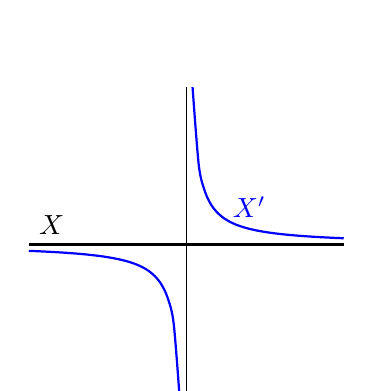
\begin{tikzpicture}[scale=0.4]
  % Axes
  \draw[-] (-5,0) -- (5,0) node[right] {};
  \draw[-] (0,-5) -- (0,5) node[above] {};

  % y = 0
  \draw[thick] (5,0) -- (-5,0) node[above right] {$X$};

  % y = 1/x (right branch)
  \draw[domain=0.2:5, smooth, thick, blue]
    plot (\x, {1/\x});

  % y = 1/x (left branch)
  \draw[domain=-5:-0.2, smooth, thick, blue]
    plot (\x, {1/\x});

  % Labels
  \node[blue] at (2,1.2) {$X'$};
\end{tikzpicture}
  \end{center}

  Let $S = k[X'] = k[x,y]/(xy - 1)$ (recall that this is the coordinate ring
  of the variety $X'$. we may also assume $k = \C$).
  By definition, $R = \pi^*(k[X])$ (where $\pi^*$ is the pullback map
  of rings induced by the map $\pi$ on the varieties),
  so that $S/R$ is a ring extension.
  Note that $\pi^*$ is not an isomorphism (since $\pi$ is not an isomorphism
  of varieties), however, it is injective, so by restricting it to its
  image we get that $\tilde \pi^* \colon k[X] \to R$ is an isomorphism.

  Next, we want to figure out if $S/R$ is an integral extension.
  The point $0 \in X$ has no source in $X'$ (geometrically, ``it has no point
  above it'').
  Algebraically, the fact $0$ has no source,
  or that the ideal at $0$ (which is $(x)$) has no ideal lying
  over it follows from \Cref{thm:lying-over} by the fact
  the equation
  \[\begin{tikzcd}[ampersand replacement=\&,cramped]
    \boxed{\phantom{x}} \& S \\
	{(x)} \& R \& {k[X]}
  \arrow["\idealin", shift right=1.5, draw=none, from=1-1, to=1-2]
	\arrow[from=2-1, to=1-1]
  \arrow["\idealin", shift right=1.5, draw=none, from=2-1, to=2-2]
	\arrow[from=2-2, to=1-2]
	\arrow["\cong"{description}, draw=none, from=2-2, to=2-3]
\end{tikzcd}\]
  has no prime solution for $\square$,
  and no solution in maximal ideas.
  Thus $S/R$ is not an integral extension.
\end{example}

\begin{theorem}[Going up]
  \label{thm:going-up}
  Let $R'/R$ be an integral extension.
  Let $P,Q \idealin R$ be prime ideals such that $P \subseteq Q$
  and let $P' \idealin R'$ be a prime ideal lying over $P$.
  Then there exists a prime ideal $Q' \idealin R'$ which is lying over $Q$
  such that $P' \subseteq Q'$.
\end{theorem}
\begin{proof}
  The kernel of the projection $R \to R' \to R'/P'$ given by
  $x \mapsto x \mapsto x + P'$ is $R \cap P' = P$.
  Thus $R/P \hookrightarrow R'/P'$ given by $x + P \mapsto x + P'$
  identifies $R/P$ with its image in $R'/P'$.
  Since $R'/R$ is integral so is $(R'/P')/R/P$.
  Thus, by \Cref{thm:lying-over},
  there exists a prime $Q'/P' \idealin R'/P'$ lying over
  $Q/P$, such that $Q'/P' \cap R/P = Q/P$,
  or equivalently $Q' \cap R = Q$.
  The proof is finished, but we add that the ``lying over'' diagram
  for convenience.
  \[\begin{tikzcd}[ampersand replacement=\&,cramped]
	{\boxed{Q'/P'}} \& {R'/P'} \\
	{Q/P} \& {R/P}
	\arrow["\normalin", draw=none, shift right=1.5, from=1-1, to=1-2]
	\arrow[from=2-1, to=1-1]
	\arrow["\normalin", draw=none, shift right=1.5, from=2-1, to=2-2]
	\arrow[from=2-2, to=1-2]
\end{tikzcd}\]
\end{proof}

\begin{example}
  Let $k = \C$, let $R = k[\A^1] = k[x]$ be identified with its image
  in $R' = k[x,y]/(xy-1) \cap (x,y)$.
  Let $X = \A^1$ and $X' = V(xy-1) \cup V(x,y) = V((xy-1) \cap (x,y))$.
  If the extension were integral, by the ``going up'' theorem,
  the ``going up diagram equation''
  \[\begin{tikzcd}[ampersand replacement=\&,cramped]
	{R'} \& {(xy-1)} \& {\boxed{\phantom{x}}} \\
	R \& {(0)} \& {(x)}
	\arrow["\subseteq", shift right=2.6, draw=none, from=1-2, to=1-3]
	\arrow[no head, from=1-3, to=2-3]
	\arrow[no head, from=2-1, to=1-1]
	\arrow[no head, from=2-2, to=1-2]
	\arrow["\subseteq", shift right=2.6, draw=none, from=2-2, to=2-3]
\end{tikzcd}\]
  has no solution,
  that is because $P' = (xy - 1) \idealin R'$ is a prime lying over $(0)$,
  and $(x,y)$ is the only prime ideal lying over $Q = (x)$,
  but $(xy - 1) \subsetneq (x,y)$.
  Hence $R'/R$ is not an integral extension.
\end{example}

\begin{example}
  Let $X = \A^1$ and $X' = \A^1 \cup \set{(0,1)} \subset \A^2$,
  with the projection map $\pi \colon X' \to X$ defined by $\pi(x,y) = x$.
  Let $Q' := (x,y-1)$ be the point ideal corresponding to $(0,1)$.
  On the level of rings, $R$ is the image of
  $k[x]$ in $R' = k[x,y]/(y) \cap (x,y-1)$.
  The corresponding ideals are $P = (0)$ and $Q = (x)$,
  and $Q' = (x,y-1)$.
  Then, the diagram equation:
  \[\begin{tikzcd}[ampersand replacement=\&,cramped]
    {R'} \& {\boxed{\phantom{P}}} \& {Q'} \\
	R \& P \& Q
	\arrow["\subseteq", shift right=2.2, draw=none, from=1-2, to=1-3]
	\arrow[no head, from=2-1, to=1-1]
	\arrow[no head, from=2-2, to=1-2]
	\arrow["\subseteq", shift right=2.2, draw=none, from=2-2, to=2-3]
	\arrow[no head, from=2-3, to=1-3]
\end{tikzcd}\]
  has no solution since:
  \begin{itemize}
    \item $Q' \cap R = (x) = Q$
    \item there is no $P' \subseteq Q'$ prime such that $P' \cap R = (0)$.
  \end{itemize}
  It follows that $R'/R$ is not an integral extension.
\end{example}

\begin{theorem}[Going down]
  Let $R'/R$ be an integral extension such that $R$ is normal (has no nilpotent
  elements) and $R'$ is an integral domain.
  Let $P \subseteq Q$ be primes in $R$ and $Q' \idealin R$ be a prime
  lying over $Q$.
  Then there exists a prime $P' \idealin R'$ such that $P' \subseteq Q'$
  lying over $P$.
  Equivalently, we have a prime solution for the following equation:
  \[\begin{tikzcd}[ampersand replacement=\&,cramped]
    {R'} \& {\boxed{\phantom{P}}} \& {Q'} \\
	R \& P \& Q
	\arrow["\subseteq", shift right=2.2, draw=none, from=1-2, to=1-3]
	\arrow[no head, from=2-1, to=1-1]
	\arrow[no head, from=2-2, to=1-2]
	\arrow["\subseteq", shift right=2.2, draw=none, from=2-2, to=2-3]
	\arrow[no head, from=2-3, to=1-3]
\end{tikzcd}\]
\end{theorem}
\begin{proof}
  Since $R'$ is an integral domain, we may identify it with its image
  in the localization $R'_{Q'}$.

  \noindent
  \textbf{Claim:} There exists a prime $P'_{Q'} \idealin R'_{Q'}$
  such that $P'_{Q'} \cap R = P$.

  \noindent
  If this claim is correct, then $P'_{Q'}$ is of the form
  $P' R'_{Q'}$ (by characterization of ideals in localized rings any ideal
  is of this form) for a prime $P' \subseteq Q'$ of $R'$
  and
  \[
    P' \cap R = \del{P'_{Q'} \cap R'} \cap R = P'_{Q'} \cap R = P,
  \]
  which completes the proof.

  \noindent
  \textbf{Proof of claim:}
  In order to prove the claim, it suffices to verify that the conditions
  for the lying over theorem (\Cref{thm:lying-over}) are satisfied,
  and ther result follows from it immediately.
  %
  The main condition we need to show is:
  \[
    P R'_{Q'} \cap R \subseteq P.
  \]
  Suppose $a \in P R' \cap R$.
  Then $a = \frac{p}{s}$ for $p \in P R'_{Q'}$ and $s \in R' \setminus Q'$.
  %
  In order to verify the condition, we will use the following
  version of Gauss' lemma:

  \begin{lemma}[Gauss' lemma]
    \label{lem:gauss}
    Let $R'/R$ be an integral extension of integral domains such that
    $R$ is normal and $P \idealin R$ is prime.
    Let $a \in P R'$ and let $f \in F[x]$ be the minimal polynomial
    of $a$ over $F = \Frac(R)$.
    Then $f \in R[x]$ and all of its coefficients
    but the leading coefficient are in $P$.
  \end{lemma}

  By Gauss' lemma the minimal polynomial of $p$ is:
  \[
    f(x) = x^n + c_{n-1} x^{n-1} + \cdots + c_0 \in R[x],
  \]
  for $c_i \in P$.
  Then
  \[
    \frac{1}{a^n} f(ax) =
    x^n + \frac{c_{n-1}}{a} x^{n-1} + \cdots + \frac{c_0}{a^n}
  \]
  is the minimal polynomial of $s \in R'$ over $F$.
  By the lemma, $c_i' := \frac{c_i}{a^{n-i}} \in R$
  or $a^{n-i} c_i' = c_i \in P$.
  Assume, by way of contradiction, that $a \notin P$,
  and the $c_i' \in P$ for all $i$.
  Thus,
  \[
    s^n = -c_{n-1}' s^{n-1} - \cdots - c'_0 \in P,
  \]
  hence $s \in P$ which is a contradiction.
  This contradiction completes the proof.
\end{proof}

% F(p) = F(s) and $F = F(a)$

\begin{exercise}[Gauss' lemma, slightly weaker version]
  \label{ex:gauss-lemma}
  Let $R$ be a normal domain and $F = \Frac(R)$ be its fraction field.
  If $g \in R[x]$ is monic, and $g = f \cdot h \in F[x]$ for a monic
  $h$, then $f,h \in R[x]$.
\end{exercise}

\begin{proofof}{\Cref{lem:gauss}}
  Write:
  \[
    p = p_1 a_1 + \cdots + p_k a_k \in P R',
  \]
  for $p_i \in P$ and $a_i \in R'$.
  Replace $R'$ by $R[a_1,\dots,a_k]$,
  a finite extension of $R$.
  
  Since $R'/R$ is a finite extension,
  we can apply the Cayley--Hamilton theorem on
  $\varphi \colon R' \to R$ defined by:
  \[
    \varphi(x) := px \in P R',
  \]
  and get that:
  \[
    \varphi^n + c_{n-1} \varphi^{n-1} + \cdots c_0 = 0,
  \]
  for some $c_i \in P$.
  We can now plug in $1$ to get
  \[
    g(p) :=
    p^n + c_{n-1} p^{n-1} + \cdots c_0 = 0.
  \]
  Since $g = f \cdot h$, and $g$ is monic,
  and $h$ is a minimal polynomial and hence monic,
  so by \Cref{ex:gauss-lemma}, $f,h \in R[x]$.

  Note that $\pmod{P}$ we have that:
  \[
    g(x) = x^n \pmod{P}.
  \]
  Thus $f \equiv x^k \pmod{P}$, and $h = x^{n-k} \pmod{P}$,
  and hence the nonleading coefficients of $f$ are in $P$,
  which completes the proof.
\end{proofof}

\newpage

\section{Noether's lemma}
\subsection{Noether's lemma}

\begin{example}
  Let $R' := \C[x_1,x_2] / (x_1 x_2 - 1)$ be the coordinate ring
  of functions on $X' = V(x_1 x_2 - 1)$,
  and let $R = \C[x_1]$ be identified with its image in $R'$.
    \begin{center}
  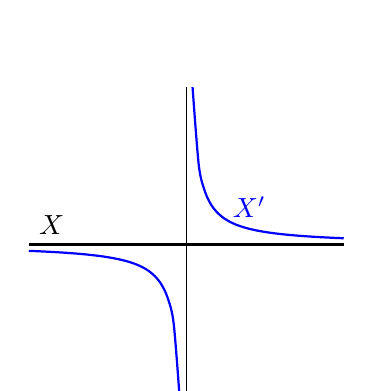
\begin{tikzpicture}[scale=0.4]
  % Axes
  \draw[-] (-5,0) -- (5,0) node[right] {};
  \draw[-] (0,-5) -- (0,5) node[above] {};

  % y = 0
  \draw[thick] (5,0) -- (-5,0) node[above right] {$X$};

  % y = 1/x (right branch)
  \draw[domain=0.2:5, smooth, thick, blue]
    plot (\x, {1/\x});

  % y = 1/x (left branch)
  \draw[domain=-5:-0.2, smooth, thick, blue]
    plot (\x, {1/\x});

  % Labels
  \node[blue] at (2,1.2) {$X'$};
\end{tikzpicture}
  \end{center}
  We have seen in \Cref{ex:lying-over} that $R'/R$ is not an integral
  extension, by the lying over theorem.
  We will show that by a change of coordinates we \textit{could}
  get an integral extension.
  The change of coordinates is:
  \begin{align*}
    x_1 &= y_1 + y_2 \\
    x_2 &= y_2 - y_1
  \end{align*}
  In these coordinates we get $R'[y_1,y_2]/(y_2^2 - y_1^2 - 1)$,
  which is integral over $R[y_1]$,
  not only because geometrically see that this is actually a projection
  of $X'$ over the following red line:
  \begin{center}
  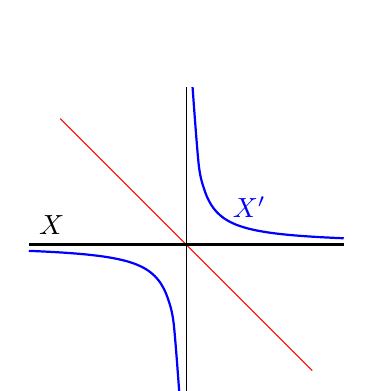
\begin{tikzpicture}[scale=0.4]
  % Axes
  \draw[-] (-5,0) -- (5,0) node[right] {};
  \draw[-] (0,-5) -- (0,5) node[above] {};
  \draw[-,red] (-4,4) -- (4,-4);

  % y = 0
  \draw[thick] (5,0) -- (-5,0) node[above right] {$X$};

  % y = 1/x (right branch)
  \draw[domain=0.2:5, smooth, thick, blue]
    plot (\x, {1/\x});

  % y = 1/x (left branch)
  \draw[domain=-5:-0.2, smooth, thick, blue]
    plot (\x, {1/\x});

  % Labels
  \node[blue] at (2,1.2) {$X'$};
\end{tikzpicture}
  \end{center}
  in which every point has a ``point over it'',
  but also because we see that it is simply the ring extension
  we get by adjoining the root of the monic polynomial
  $x^2 - y_1^2 - 1 \in \C[y_1][x]$.
\end{example}

\begin{remark}[Goal]
  Given a finitely generated $k$-algebra $R'$,
  our next goal is to find a subring $R$ such that
  $R \cong k[z_1,\dots,z_r]$ and $R'/R$ is finite.
\end{remark}

\begin{definition}[Total degree of a monomial]
  Let $x_1^{a_1} x_2^{a_2} \cdots x_r^{a_r}$ be a monomial.
  We define its total degree to be
  \[
    \td(x_1^{a_1} x_2^{a_2} \cdots x_r^{a_r}) = a_1 + a_2 + \cdots + c_r.
  \]
\end{definition}

\begin{definition}[Total dergee of a polynomial]
  The total degree of a polynomial
  is defined to be the maximal total degree of its monomials.
\end{definition}

\begin{definition}[Homogeneous polynomial]
  A polynomial $p \in k[x_1,\dots,x_r]$ is called homogeneous
  if all of its monomials have the same total degree.
\end{definition}

\begin{remark}
  
\end{remark}

\begin{lemma}
  \label{lem:nonzero}
  Let $0 \neq f \in k[x_1,\dots,x_n]$ be homogeneous polynomial
  over an infinite field $k$.
  Then there exist $a_1,\dots,a_{n-1}$ such that
  $f(a_1,\dots,a_{n-1},1) \neq 0$.
\end{lemma}
\begin{proof}
  We simply prove this by induction on $n$.
  In the base case $n = 1$ we have $f(x_1) = c x_1^k$, for $c \neq 0$,
  and then $f(1) = c \neq 0$.
  Next we suppose the claim holds for all $n > k \geq 1$,
  and show the claim for $n$.
  Write $f$ as a ``polynomial in $x_1$'' as follows:
  \[
    f(x_1,\dots,x_n) =
    \sum_{i=0}^{d} f_i(x_2,\dots,x_n) x_1^i,
  \]
  where $f_i$ is homogeneous of degree $d - i$ or $f_i \equiv 0$.
  Since $f \neq 0$, we get $f_m \neq 0$ for some $0 \le m \le d$.
  By induction, there exist $a_2,\dots,a_{n-1} \in k$
  such that its dehomogenization in the last coordinate is nonzero:
  \[
    f_m(a_2,\dots,a_{n-1},1) \neq 0,
  \]
  and hence the polynomial
  \[
    0 \neq f(x,a_2,\dots,a_{n-1},1) \in k[x]
  \]
  is a polynomial, with finitely many roots
  (and it is not the zero polynmial).
  Since $k$ is infinite, there exists $a_1 \in k$ such that
  \[
    f(a_1,a_2,\dots,a_{n-1},1) \neq 0,
  \]
  which completes the proof.
\end{proof}

\begin{lemma}
  \label{lem:nother-lem-lem}
  Let $0 \neq f \in k[x_1,\dots,x_n]$ be a polynomial
  over an infinite field.
  Then there exists $a_1,\dots,a_{n-1},\lambda \in k$
  and a change of coordinates
  such that:
  \[
    \lambda f(y_1 + a_1 y_n, y_2 + a_2 y_n, \dots, y_{n-1} + a_{n-1} y_{n-1},y_n) \in k[y_1,\dots,y_n],
  \]
  is monic in $y_n$.
\end{lemma}
\begin{proof}
  Let $d$ be the the total degree of $f$ and write:
  \[
    f = \sum_{k_1,\dots,k_n} c_{k_1,\dots,k_n} x_1^{k_1} \cdots x_n^{k_n},
  \]
  such that $c_{k_1,\dots,k_n} \in k$.
  Then:
  \begin{multline*}
    \lambda f(y_1 + a_1 y_n, y_2 + a_2 y_n,
      \dots, y_{n-1} + a_{n-1} y_{n-1},y_n) \\
    = \sum_{k_1,\dots,k_n} c_{k_1,\dots,k_n}
      (y_1 + a_1 y_n)^{k_1} \cdots
      (y_{n-1} + a_{n-1} y_n)^{k_{n-1}} y_n^{k_n}.
  \end{multline*}
  The leading coefficient is:
  \[
    \lambda \sum_{k_1 + \cdots + k_n = d}
    c_{k_1,\dots,k_n} a_1^{k_1} \cdots a_{n-1} k^{n-1} \cdot y_n^{k_1 + \cdots + k_n} \cdot 1^{k_n}
    = \lambda f_d(a_1,\dots,a_{n-1},1) y_n^d,
  \]
  for a homogeneous polynomial $f_d \neq 0$ of degree $d$.
  By \Cref{lem:nonzero} we can pick $a_1,\dots,a_{n-1} \in k$
  (remember they were free variables so far)
  such that $f_d(a_1,\dots,1) \neq 0$,
  and the claim follows by picking $\lambda = 1/f_d(a_1,\dots,a_{n-1},1)$.
\end{proof}

\begin{lemma}[Noether's lemma]
  Let $R$ be a finitely generated $k$-algebra.
  Then there exists an injective homomorphism
  $i \colon k[z_1,\dots,z_r] \to R$ such that
  $R / \im(i)$ is a finite extension.
\end{lemma}
\begin{proof}
  Suppose that $R$ is generated over $k$ by $x_1,\dots,x_n$.
  We prove this lemma by induction on $n$.
  In the base case $n = 0$ we haev $R = k$ and the claim is immediate.
  Suppose $n > 0$.

  \noindent
  \textbf{Case I:} $x_1,\dots,x_n$ are algebraically independent.
  In this case $i \colon k[z_1,\dots,z_n] \to R$ defined by $i(z_i) = x_i$
  is an isomorphism, which completes the proof.

  \noindent
  \textbf{Case II:} $x_1,\dots,x_n$ are not algebraically independent.
  In this case suppose $f \neq 0$ is a polynomial in $n$ variables
  such that $f(x_1,\dots,x_n) = 0 \in R$.
  As in \Cref{lem:nother-lem-lem}, we pick $a_1,\dots,a_{n-1},\lambda$
  such that if:
  \begin{align*}
    y_1 &= x_1 - a_1 y_n \\
        &\vdotswithin{=} \\
    y_{n-1} &= x_{n-1} - a_{n-1} y_n \\
    y_n &= x_n,
  \end{align*}
  then $R = k[y_1,\dots,y_n]$ and now:
  \[
    \lambda f(y_1 + a_1 y_n, y_2 + a_2 y_n, \dots, y_{n-1} + a_{n-1} y_{n-1},y_n) \in k[y_1,\dots,y_n],
  \]
  is a monic polynomial in $y_n$.
  Thus, $R = k[y_1,\dots,y_n]$ is a finite extension of $k[y_1,\dots,y_{n-1}]$.
  By induction, $k[y_1,\dots,y_{n-1}]/k[z_r,\dots,z_r]$ is a finite
  extension, for some subalgebra $k[z_r,\dots,z_r]$ isomorphic to a polynomial
  ring.
  Since both the first extension $k[y_1,\dots,y_n]/k[y_1,\dots,y_{n-1}]$
  and the second extension $k[y_1,\dots,y_{n-1}]/k[z_r,\dots,z_r]$ are finite,
  then we conclude that $R/k[z_1,\dots,z_r]$ is finite,
  which completes the proof.
\end{proof}

\subsection{More nullstellensatzs}

\begin{corollary}[Algebraic version of the weak nullstellensatz]
  \label{cor:algebraic-version-of-the-weak-null}
  Let $R$ be a finitely generated $k$-algebra.
  If $R$ is a field, then $R/k$ is a finite field extension.
\end{corollary}
\begin{proof}
  By Noether's lemma, $R$ is a finite extension of a polynomial
  ring $k[z_1,\dots,z_r]$ in variables $z_1,\dots,z_r$.
  The following diagram is just for visual aid for the following
  and last part of the proof:

  \[\begin{tikzcd}[ampersand replacement=\&,cramped]
    R \& {\boxed{\phantom{R}}} \\
    {k[z_1,\dots,z_r]} \& p \\
    k
    \arrow[no head, from=2-1, to=1-1]
    \arrow["{\rotatebox{90}{=}}", draw=none, shift right=2, from=3-1, to=2-1]
  \end{tikzcd}\]

  Since $R/k[z_1,\dots,z_r]$ is finite,
  by the lying over theorem, there is no nontrivial
  prime ideal in $k[z_1,\dots,z_r]$.
  But $k[z_1,\dots,z_r]$ is a polynomial ring!
  This implies that $r = 0$ and $R/k$ is finite.
\end{proof}

\begin{remark}
  \label{rem:null}
  If $k = \overline k$, then $R/k$ cannot be finite
  unless $R = k$, and thus we get $R = k$.
\end{remark}

\begin{corollary}[Nullstellensatz, weak version]
  Let $k = \overline k$ be an algebraically closed field.
  Then every maximal ideal $M$ in a polynomial ring $R = k[x_1,\dots,x_n]$
  is a point ideal $M = I(\vec a) = (x_1 - a_1, x_2 - a_2, \dots, x_n - a_n)$,
  for some $\vec a = (a_1,\dots,a_n) \in \A_k^n$.
\end{corollary}
\begin{proof}
  Let $M \idealin k[x_1,\dots,x_n]$ be a maximal ideal.
  Then $R/M$ is a field.
  But $R/M$ is also a finitely generated $k$-algebra
  with the homomorphism $\varphi \colon k \to R/M$
  defined by $\varphi(\alpha) = \alpha + M$.
  (then $R/M$ is generated by the finitely many $\bar x_i = x_i + M$).

  Since $k = \overline k$, by the algebraic version of the nullstellensatz
  and \Cref{rem:null} we have $R/M \cong \im(\varphi)$,
  so $\varphi$ is an isomorphism.
  Let $a_i \in k$ be $\varphi^{-1}(\bar x_i)$.
  Then $\bar x_i = \bar a_i$, which equivalently means that $x_i - a_i \in M$
  for all $i$,
  and hence $I(\vec a) = (x_1 - a_1, \dots, x_n - a_n) \subseteq M$.
  We have seen that $I(\vec a)$ is maximal, and hence $M = I(\vec a)$.
\end{proof}

\begin{remark}
  We have seen before that $I$ is geometric if and only if it is radical.
  The strong formulation of the nullstellensatz is as follows.
\end{remark}

\begin{theorem}[Nullstellensatz strong form]
  \label{thm:null-algebraic-form}
  Let $X \subseteq \A_k^n$ be a variety and $I \idealin k[X] = R$.
  Then $I(V(I)) = \sqrt{I}$.
  In particular, if $I$ is radical, it is geometric.
\end{theorem}

\begin{theorem}[Algebraic version of the strong nullstellensatz]
  Let $R$ be a finitely generated $k$-algebra,
  and $I \properideal R$.
  Then $\sqrt{I} = \bigcap_{P \supseteq I \text{ max}} P$.
\end{theorem}
\begin{remark}
  Recall that the algebraic form of the strong nullstellensatz
  implies the strong nullstellensatz.
  We will show this under the additional assumption
  of the strong nullstellensatz which is $k = \overline k$.

  Let $f \in \sqrt{I}$.
  This implies that $f^n \in I$ for some $n \geq 1$ so
  $f^n(a) = 0$ for all $a \in V(I)$,
  and then $f \equiv 0$ on $V(I)$ so $f \in I(V(I))$.

  On the other hand if $f \notin \sqrt{I}$,
  by the algebraic version of the nullstellensatz there exists
  a maximal ideal $I \subseteq P \properideal R$
  such that $f \notin P$.
  By the weak nullstellensatz (which we can use since $k = \overline k$),
  \[
    P = I(a) = (x_1 - a_1,\dots,x_n - a_n),
  \]
  for some $a = (a_1,\dots,a_n) \in X \subseteq \A^n$.
  Since $I \subseteq I(a)$, we have $a \in V(I)$.
  Since $f \notin I(a)$, we have $f(a) \neq 0$
  and $f \notin I(V(I))$.
\end{remark}

\begin{proofof}{\Cref{thm:null-algebraic-form}}
  Recall that we need to show that
  $\sqrt{I} = \bigcap_{P \supseteq I \text{ max}} P$.

  First let $f \in \sqrt{I}$, we get $f^n \in I$
  so $f^n \in P$ but $P \supseteq I \text{ max}$
  is prime so $f \in P$ for all such $P$,
  so $f \in \bigcap_{P \supseteq I \text{ max}} P$.

  On the other hand (we use the Rabinowich trick),
  suppose $f \in R \setminus \sqrt{I}$.
  Let:
  \[
    S := \set{1,f,f^2,\dots}
  \]
  be a multiplicative set,
  and let $R_{f} = S^{-1}R$ be the localization at $S$.
  Since $f \notin \sqrt{I}$, we have $I \cap S = \emptyset$,
  and by an exercise from the homework,
  there exists a prime $I \subseteq P \idealin P$ such
  that $P \cap S = \emptyset$
  and:
  \[
    P_f = S^{-1} P = \set{\frac{p}{f^i} \bmid p \in P \stand i \geq 0}
  \]
  is a maximal ideal in $R_f$.
  Since $P$ is a prime, $R/P$ is an integral domain.
  Thus $R/P$ can be identified with its image in $(R/P)_f$
  since $(R/P)_f \cong R_f/P_f$ and $P_f \idealin R_f$
  is maximal, $(R/P)_f$ is a field.

  Since $R/P$ and hence $(R/P)_f$ is a finitely generated $k$-algebra,
  the algebraic version of the weak nullstellensatz
  (\Cref{cor:algebraic-version-of-the-weak-null})
  implies that $(R/P)_f/k$ is a finite extension.
  Thus, $(R/P)/k$ is a finite extension and hence $R/p$
  is a field.
\end{proofof}

\newpage

\section{Noetherian rings}
\subsection{Noetherian rings}

\begin{definition}[Noetherian module]
  Let $M$ be an $R$-module.
  Then $M$ is called Noetherian if every chain:
  \[
    M_0 \subseteq M_1 \subseteq \cdots \subseteq \cdots
  \]
  of submodules of $M$ stabilizes,
  that is, $M_i = M_{i+1}$ for all $i > i_0$
  for some $i_0$.
\end{definition}

\begin{definition}[Noetherian ring]
  A ring is $R$ is called Noetherian if $R$ is Noetherian
  as an $R$-module.
\end{definition}

\begin{remark}
  $R$ is Noetherian if and only if every ascending chain of ideals
  stabilizes.
\end{remark}

\begin{example}
  The following are Noetherian modules:
  \begin{enumerate}
    \item[(1)] All fields $k$.
    \item[(2)] A vector space $V$ over $k$ is Noetherian if and
      only if $\dim V < \infty$.
  \end{enumerate}
\end{example}

\begin{example}
  The ring $R[x_1,x_2,\dots] := \bigcup_{n \in \N} k[x_1,\dots,x_n]$
  is not Noetherian.
  We have the infinite chain:
  \[
    (x_1) \subsetneq (x_1,x_2) \subsetneq \cdots
  \]
\end{example}

\begin{lemma}
  Let $M$ be an $R$-module.
  Then the following are equivalent:
  \begin{enumerate}
    \item[(1)] $M$ is Noetherian.
    \item[(2)] Every nonempty family of submodules has a maximal element.
    \item[(3)] Every submodule of $M$ is finitely generated.
  \end{enumerate}
\end{lemma}
\begin{proof}
  It is clear that $(1) \to (2)$ is just Zorn's lemma.
  In order to show $(2) \to (3)$,
  Let $N \leqslant M$ be a submodule.
  If $N \neq 0$, pick $0 \neq x_1 \in N$ and define
  $N_1 = \langle x_1 \rangle$.
  If $N_1 \setminus N$, pick $x_2 \in N \setminus N_1$,
  and define $N_2 = \langle x_1, x_2 \rangle$.
  If the process doesn't stop, we will get an infinite increasing
  chain of submodules with no maximal element, in contradiction
  to our assumption $(2)$.
  Thus, the process must eventually stop, which implies that
  $N = N_i$ for some $i$, and hence $M$ is finitely generated.
  In order to show $(3) \to (1)$,
  let
  \[
    M_1 \subsetneq M_2 \subsetneq \cdots
  \]
  the union $M_{\infty} = \bigcup_{i=1}^{\infty} M_i$
  is a submodule, and hence it is finitely
  generated.
  Since each $x_i$ is contained somwhere in the chain,
  there exists some $i_0$ such that all generators
  are in $M_i$, hence $M_i = M_{\infty}$,
  hence the sequence stabilizes eventually so $M$ is
  Noetherian.
\end{proof}

\begin{remark} \phantom{}
  \begin{enumerate}
    \item[(1)] If $R$ is Noetherian,
      every $I \idealin R$ is finitely generated.
    \item[(2)] If $R$ is Noetherian and $J \idealin R$,
      then $R/J$ is Noetherian (Ideals in $R/J$ are of the form $I/J$
      for $J \subseteq I \idealin R$).
  \end{enumerate}
\end{remark}

\subsection{Hilbert's basis theorem}

\begin{theorem}[Hilbert's basis theorem, 1890]
  Let $R$ be a Noetherian ring.
  Then any polynomial ring $R[x]$
  is also Noetherian.
\end{theorem}
\begin{proof}
  Assume, by way of contradiction, that $R[x]$ is not Noetherian.
  Thus, there exists an ideal $I \idealin R[x]$ which is not finitely
  generated.
  Pick a sequence $f_1,f_2,\dots$ such that $f_{k+1}$ is a polynomial
  of minimal degree in $I$ but not in $(f_1,\dots,f_k)$ for all $k$.
  In particular, the sequence of degrees:
  \[
    d_1 = \deg f_1 \le d_2 = \deg f_2 \le d_3 \le \cdots
  \]
  is not decreasing.
  Write:
  \[
    f_k = a_k x^{d_k} + (\text{lower term}).
  \]
  Since $R$ is Noetherian, the sequence:
  \[
    (a_1) \subseteq (a_1,a_2) \subseteq \cdots
  \]
  stabilizes from some index $s \in \N$.
  Thus, $a_{s+1} = c_1 a_1 + \cdots c_s a_s$
  for some $c_i \in R$.
  Then the leading coefficient of $x^{d_{s+1}}$
  \[
    c_1 f_1 x^{d_{s+1} - d_1} + \cdots + c_s f_s x^{d_{s+1}-d_s} \in I
  \]
  is $c_1 a_1 + \cdots c_s a_s = a_{s+1}$.
  Thus,
  \[
    f_{s+1}' :=
    f_{s+1} - 
    c_1 f_1 x^{d_{s+1} - d_1} - \cdots - c_s f_s x^{d_{s+1}-d_s} \in I
  \]
  is of smaller degree
  but $f_{s+1}' \notin (f_1,\dots,f_s)$
  since $f_{s+1 \notin (f_1,\dots,f_s)}$.
\end{proof}

\begin{corollary}
  Every finitely generated ring $S$ over a Noetherian
  ring $R$ is Noetherian.
  In particular, the polynomial ring
  $R[x_1,\dots,x_n]$ is Noetherian.
\end{corollary}
\begin{proof}
  Suppose $S = R[z_1,\dots,z_k]$ with some relations
  between the $z_i$.
  Then there exists an epimorphism
  $\pi \colon R[x_1,\dots,x_k] \to R[z_1,\dots,z_k] = S$
  defined $x_i \mapsto z_i$,
  and $S \cong R[x_1,\dots,x_k]/\ker \pi$.
  Now since $R[x_1,\dots,x_k]$ (the variables have no relations)
  is Noetherian (by applying Hilbert's basis theorem $k$ times),
  so is its quotient $S$.
\end{proof}

\begin{corollary}
  Every finitely generated $k$-algebra
  is Noetherian.
  In particular $k[X]$ is Noetherian for $X \subseteq A_k^n$
  a variety.
  Moreover, any subvariety $Y \subseteq X$ is the zero locus
  of finitely many functions in $k[X]$.
  Equivalently, we have $I_X(Y) = (f_1,\dots,f_r)$.
  In fact every sequence of subvarieties:
  \[
    Y_0 \supseteq Y_1 \supseteq \cdots
  \]
  stabilizes since it corresponds to
  $I(Y_0) \subseteq I(Y_1) \subseteq \cdots$.
\end{corollary}

\begin{remark}[Artinian ring]
  An Artinian ring is a notion equivalent to a Noetherian
  ring where the chains are decreasing instead of decreasing.
  This is a much stronger condition and not as many rings are Artinians.
  In commutative algebra we even have that any Artinian ring is also Noetherian.
  This notion is less relevant in this course, and is studied
  more throughouly in noncommutative algebra.
\end{remark}

\begin{remark}
  Recall definitions of dimension discussed in the previous sections.
\end{remark}

\begin{example}
  If $R = k$ is a field, then $\dim R = 0$
  since the longest sequence of primes is $(0)$.
\end{example}

\begin{example}
  If $R$ is a PID (for example $k[x]$ but not $k[x,y]$)
  but not a field, then $\dim R = 1$.
  The maximal chain is $(0) \subsetneq M$ where $M$ is maximal.
  We also have that $\dim R[x_1,\dots,x_n] = n$
  and $\dim \A_k^n = n$,
  and the following theorem will show this.
\end{example}

\begin{theorem}
  \label{thm:dimension}
  Every maximal chain of primes:
  \[
    C := (P_0 \subsetneq P_1 \subsetneq \cdots \subsetneq P_m)
  \]
  in $k[x_1,\dots,x_n]$ is of length $m = n$.
  In particular $\dim k[x_1,\dots,x_n] = n$.
\end{theorem}

\begin{exercise}
  \label{ex:dim-one}
  In a Noetherian UFD $R$ every minimal prime
  ideal is principle.
\end{exercise}

\begin{exercise}
  \label{ex:dim-two}
  Given an integral extension of finitely generated $k$-algebras
  and prime ideals $P_1$,$P_2$,$P_3$,$Q_1$,$Q_2$ as in (diagram to be added),
  then there exists $Q_1 \subsetneq Q_2 \subsetneq Q_3$.
\end{exercise}

\begin{lemma}[Incomparability lemma]
  \label{lem:incomparability-lemma}
  If $R'/R$ is integral and $P \idealin R$ and $P',Q' \idealin R'$
  are ideals lying over $P$.
  Then $P' \supsetneq Q'$.
\end{lemma}

\begin{proofof}{\Cref{thm:dimension}}
  By induction on $n$.
  For $n = 0$ or $n = 1$ see examples from earlier. % (add references).
  We claim that in the chain $C$ we have $m = n$.
  Since $C$ is maximal, $P_0 = (0)$ and $P_1$ is a minimal prime,
  and $P_m$ is maximal.

  By \Cref{ex:dim-one}, we have $P_1 = (f)$
  for some $0 \neq f \in k[x_1,\dots,x_n]$.
  Let $R' := k[x_1,\dots,x_n]/p_1$,
  and $R := k[x_1,\dots,x_{n-1}]$.
  Then the chain of primes:
  \[
    (0) = P_1/P_1 \subsetneq P_2/P_1 \subsetneq P_m/P_1
  \]
  is lying over
  \[
    (0) = P_1/P_1 \cap R \subsetneq P_2/P_1 \cap R \subsetneq P_m/P_1 \cap R.
  \]
  By a change of variables using  Noether's lemma
  we can assume $f$ is monic in $x_n$.
  Thus we get that $R'/R$ is integral and the map from $R$ to $R'$ is injective,
  so we can use the incomparability lemma to get that $P_i/P_1$ and $P_{i+1}/P$
  are not lying over the same prime, so $R \cap P_i/P_1 \subsetneq R \cap P_{i+1}/P_1$
  for all $i$.
  Now we can conclude that
  \[
    (0) = P_1/P_1 \cap R \subsetneq P_2/P_1 \cap R \subsetneq P_m/P_1 \cap R
  \]
  is a maximal chain by the second exercise plus the going up theorem
  (note that the length of this chain is $m-1$ not $m$ since earlier we defined
  $m$ to be the length of $C$ which going from $P_0$ to $P_m$).
  Thus by induction we conclude that $m - 1 = n - 1$,
  so $m = n$ which completes the proof.
\end{proofof}

\begin{proofof}{\Cref{lem:incomparability-lemma}}
  Assume on the contrary that $P' \subseteq Q'$,
  and $a \in Q' \setminus P'$.
  Since $R'/P'$ is integral over $R/P$,
  the element $\overline a \in R'/P'$ satisfies:
  \[
  \overline a^n + \overline{c}_{n-1} \overline a^{n-1} + \cdots +
    \overline c_0 = 0,
  \]
  for some $c_i \in R$.
  Assume that this polynomial that vanishes on $\overline a$
  has minimal degree.
  Since $\overline a \in Q'/P'$,
  \[
    \overline{c_0} =
    - \overline a^n - \cdots - \overline{c}_1 \overline a \in Q'/P',
  \]
  and hence $c_0 \in Q' \cap R = P$, so $\overline{c_0} = 0$.
  Since $R/P$ is an integral domain we get that:
  \[
    \overline a^{n-1} + \cdots + \overline{c_1} = 0,
  \]
  which contradicts the minimality we assumed previously,
  and completes the proof.
\end{proofof}

\begin{exercise}
  Let $R = \C[x]$ and $R' = \C[x,y,z]/(z^2-y^3)$.
  Check if $R'/R$ is integral.
\end{exercise}
\begin{solution}
  We have that both $(x)$ and $(x,y,z)$ are lying over $(x)$,
  and thus by the incomparability lemma $R'/R$ cannot be integral.
\end{solution}

\begin{remark}
  Our next goal is to find the dimension of $k[x_1,\dots,x_n]/P$
  for any prime ideal $P$.
\end{remark}

\begin{definition}[Height of an ideal]
  The codimension (or height) of a prime ideal $P \idealin R$
  is:
  \[
    \codim_R(P) :=
      \sup\set{n \bmid
        \text{there exists $P = P_n \supsetneq \cdots \supsetneq P_0$
        of length $n$}}.
  \]
\end{definition}

\begin{remark}
  The height of an ideal could potentially be $\infty$.
\end{remark}

\begin{definition}[Codimension of a subvariety]
  For an irreducible subvariety $Y \subseteq X$,
  we define the codimension of $Y$ by:
  \[
    \codim Y := \codim_{k[X]} I_X(Y).
  \]
\end{definition}

\begin{remark}
  This is the maximal length of a chain of irreducible subvarieties:
  \[
    Y = Y_n \subsetneq \cdots \subsetneq Y_0 \subseteq X.
  \]
\end{remark}

\begin{proposition}
  \label{prop:dimension-of-quotient}
  Let $R$ be a ring of dimension $n$ such that every maximal chain of
  prime ideals if of length $n$.
  Let $P \idealin R$ be a prime.
  Then:
  \[
    \dim R = \codim_R P + \dim R/P.
  \]
  Moreover, every maximal chain of primes in $R/P$
  is of length $\dim R - \codim P$.
\end{proposition}
\begin{proof}
  Every maximal chain of prime ideals in $R/P$ corresponds to a maximal
  chain of primes:
  \[
    P = Q_0 \subsetneq \cdots \subsetneq Q_r \subseteq R,
  \]
  in $R$.
  By definition of $s = \codim_R P$, there exists a maximal chain:
  \[
    P = P_s \supsetneq \cdots \supsetneq P_0.
  \]
  Thus,
  \[
    \underbrace{P_0 \subsetneq \cdots \subsetneq P_s}_{\codim_R P} =
    P =
    \underbrace{Q_0 \subsetneq \cdots \subsetneq Q_r \subseteq R}_{\dim R/P}
  \]
  us a maximal chain in $R$.
  Thus, its length is $n = \dim R = r + s$.
  In total,
  we have that $\dim R \geq \dim R/P + \codim_R P \geq p + s = \dim R$.
  Thus all inequalities are actually equalities,
  and every maximal chain in $R/P$ is of length $\dim R/P$.
\end{proof}

\begin{exercise}
  Let $X = V(x^2 + y^2 - 1) \subseteq \A_k^2$ for an algebraically
  closed field $k = \overline k$.
  Show that $\dim k[X] = 1$.
\end{exercise}
\begin{solution}
  Our variety is of the shape:
  \begin{center}
    \begin{tikzpicture}
      \draw[very thick] (90:1) arc[start angle=90, end angle=-270, radius=1];
      \draw[-->] (-3, 0) -- (3, 0) node[right] {$x$};
      \draw[-->] (0,-1.5) -- (0,1.8) node[right] {$y$};
    \end{tikzpicture}
  \end{center}
  Since $P = (x^2 + y^2 - 1) \idealin k[x,y]$ is prime,
  thus,
  \[
    \set{0} \subsetneq P = (x^2 + y^2 - 1) \subsetneq (y, x - 1) =: m
  \]
  is a maximal chain of primes in $k[x,y]$.
  Thus,
  \[
    \set{0} = P/P \subsetneq m/p
  \]
  is a maximal chain in $R/P$,
  and we conclude that $\dim R/P = 1$.
  We then compute using \Cref{prop:dimension-of-quotient}
  that:
  \[
    \codim P = \dim R - \dim R/P = 2 - 1 = 1.
  \]
\end{solution}

\begin{corollary}
  For every finitely generated $k$-algebra $R$,
  which is an integral domain,
  all maximal chains of primes are of the same length $\dim R$.
\end{corollary}
\begin{proof}
  If $R = k[z_1,\cdots,z_n]$ (where the $z_i$ may have relations),
  there exists $\varphi k[x_1,\dots,x_n] \to R$
  given by $x_i \mapsto z_i$
  whose kernel $P = \ker \varphi$ is a prime
  (since $k[x_1,\dots,x_n]/P \cong R$ which is an integral domain).
  Now the claim follows from the proposition (add reference).
\end{proof}

\begin{example}
  In $R = k[x,y] / (y) \cap (x, y - 1)$
  both $(x, y - 1)$ and $(y) \subsetneq (x,y)$ are maximal chains.
\end{example}


\subsection{Noetherian normalization}

\begin{definition}[Noetherian normalization]
    Given $\dim X = \dim k[x_1,\dots,x_n]/I(X)$
    we finnd $k[X]/k[y_1,\dots,y_m]$ finite
    then $\dim X = m$.
\end{definition}

\begin{example}
    Let $X = V(y^2 - x^2) \subseteq \A^2$
    and $R' = k[X] = k[x,y]/(y^2-x^2)$
    and $R = k[\A^1]$
    is the coordinate projection of the variety
    onto $\A^1$.
    The resulting $R'/R$ is an integral extension
    with $\dim R' = \dim R$.

Proof $\dim R' \geq \dim R$:
Given a maximal chain $P_0 \subsetneq \cdots \subsetneq P_n$ of primes in $R$,
we may pick $Q_0$ to be a prime over $P_0$ by
``lying over''.
By going up we may choose primes $Q_1,\dots,Q_n$
lying over $P_1,\dots,P_n$ respectively such that
$Q_0 \subsetneq Q_1 \subsetneq \cdots \subsetneq Q_n$,
which completes the first direction of the proof.


In order to show the other direction let
$Q_0 \subsetneq \cdots \subsetneq Q_n$
be a chain of primes in $R'$.
We define $P_i := Q_i \cap R$ a chain of rising
ideals in $R$ below $Q_i$.
By the incomparability lemma $P_{i+1} \neq P_i$
for all $i$ so $P_0 \subsetneq \cdots \subsetneq P_n$
is a chain of primes of length at least $n$,
which completes the second direction and completes
the proof.
\end{example}

\begin{corollary}
    Let $R$ be a finitely generated $k$-algebra,
    and $i \colon k[x_1,\dots,x_n] \hookrightarrow R$
    a Noetherian normalization.
    Then $\dim R = n$.
\end{corollary}
\begin{proof}
    In a Noetherian normalization
    $R / i(k[x_1,\dots,x_n])$ is integral
    and hence by the previous proposition
    $\dim R = \dim k[x_1,\dots,x_n] = n$.
\end{proof}

\begin{remark}
    In particular, the number
    of variables in any two Noetherian normalizations
    is the same.

    \textbf{Recall:} (definition of transcendence
    degree) For a finitely generated field extension
    $E/K$ we define $\trdeg_K E$ to be
    the maximal number of algebraically independent
    elements over $K$.
\end{remark}

\begin{corollary}
Let $R$ be a finitely generated $k$-algebra
such that $R$ is an integral domain,
and $F = \Frac(R)$ its fraction field.
Then $\dim R = \trdeg_K F$.
\end{corollary}
\begin{proof}
Let $k[x_1,\dots,x_n] \hookrightarrow$ be a Noetherian
normalization.
From the second to last corollary $\dim R = n$.
Since $R/k[x_1,\dots,x_n]$ is integral,
$F/k(x_1,\dots,x_n)$ is algberaic
and hence $\trdeg F = \trdeg k(x_1,\dots,k_n) = n = \dim R$.
\end{proof}

\newpage

\section{Tangent spaces}

\subsection{Introduction and Nakayama's lemma}

Let $X \subseteq \A^n$ be a variety
and $\bar a = (a_1,\dots,a_n) \in X$.
For $f \in k[x_1,\dots,x_n]$,
we can define the \textit{formal derivative}
with respect to $x_i$ just like we did in field
theory (the definition coincide with standard polynomial
differentiation).

We also define the formal differential
$\dif \colon k[x_1,\dots,x_n] $
by:
\[
    f \mapsto \dif_a f := \sum \frac{\partial f}{\partial x_i}(\bar a) y_i
\]
where $y_i = x_i - a_i$ for $i=1,\dots,n$.
The tangent space at $\bar a$ is
\[
    T_a X = V\del{\set{\dif_a f \mid f \in I(a)}}.
\]

\begin{remark}
    Writing $I(X) = (f_1,\dots,f_r)$
    one has $T_a X = V(\df_1,\dots,\df_r)$.
    This follows since for any $f,g \in I(X)$
    and $h \in k[X]$ we have $\dif_a(f + g) = \dif_a f + \dif_a g$ and $\dif_a(hf) = h(\bar a) \dif_a f + f(\bar a) \dif_a h = h(\bar a) \dif_a f$.
\end{remark}

\begin{lemma}
    Set $P = I_X(a)$.
    Then $\Hom(T_a X,k)$ (in the category $\Vect_k$)
    which is $(T_a X)^*$ is isomorphic to $P/P^2$
    as a vector space over $k[X]/P \cong k$.
\end{lemma}
\begin{proof}
    Consider $\varphi \colon P \to \Hom(T_a X,k)$
    by $f \mapsto \dif_a f\vert_{T_a X}$.
    $\varphi$ is well defined (exercise) and surjective
    ($\dif$ is surjective).
    It is left to show that $\ker \varphi = P^2$.

    For any $h_1,h_2 \in I_X(a)$ we clearly
    have $\frac{\partial (h_1 h_2)}{\partial x_i} = 0$
    which shows $\ker \varphi \supseteq P^2$.

    In the other direction for $\bar f \in P \subseteq k[X]$ such that $\dif_a f\vert_{T_a X}$.
    We claim that $\dif f = \dif g$ for some
    $g \in I(X)$,
\end{proof}

%% Continutation of tangent spaces

\begin{remark}
  Recall that if $V(f_1,\dots,f_r) = X \subseteq \A^n$ is a variety,
  we define the tangent space by $T_a X = V(\dif f_1,\dots, \dif f_r)$.

  We have seen that $\Hom(T_a X,k) = P/P^2$ where $P$ is the maximal ideal
  at the point $a$, that is, $P = I_X(a) \idealin k[X]$.
\end{remark}

\begin{proposition}
  Let $R$ be a ring (for example $k[X]$ for some variety $X$),
  with a maximal $P \idealin R$ (for example $I_X(a)$).
  Set $R_p = S^{-1} R$ where $S = R \setminus P$.
  Similarly, we can consider $S^{-1} P / S^{-1} P^2 \in R_p$-$\cmod$.
  We claim that $S^{-1} P / S^{-1} P^2 \cong P/P^2$ as $k$-vector spaces
  where $k = R/P$.
\end{proposition}
\begin{proof}
  We know that $M = P/P^2$ is an $R$-module,
  with a trivial $P$-action and hence a module over $R/P = k$,
  or since $k$ is a field, a vector space.
  Since the image of $S$ in $k = R/P$ consists of invertible elements,
  \[
    S^{-1} M =
    \underbrace{S^{-1} k}_{=\,k} \otimes M \cong M,
  \]
  as a $k$-vector space (the equality $S^{-1} k = k$ follows from 
  the fact $k$ is a field).
  Thus,
  \[
    M \cong S^{-1} M \cong S^{-1} P / S^{-1} P^2,
  \]
  as $k$-vector spaces.
\end{proof}

\begin{definition}[(co)tangent spaces]
  For a Noetherian
  local ring $R$ with a maximal ideal $P \idealin R$ and residue field
  $k = R/P$, its cotangent space is $\Hom(T_a X,k) \cong P/P^2$,
  and its tangent space is the dual $\Hom(P/P^2,k)$,
  and its dimension is $\dim_k P/P^2$.
\end{definition}

\begin{proposition}
  \label{prop:we-need-nakayama}
  For a local Noetherian ring $R$ with a maximal $P \idealin R$ 
  and residue field $k = R/P$ with have the following:
  \begin{enumerate}
  \item[(1)] $\dim_K P/P^2$ is the minimal size of a set of generators of $P$.
  \item[(2)] $\dim R \le \dim_k P/P^2$.
  \end{enumerate}
\end{proposition}

\begin{definition}[Frattini subgroup]
  Mentioned by name, to be added.
\end{definition}

\begin{lemma}[Nakayama's lemma]
  \label{lem:nakayama}
  Let $R \neq 0$ be a local ring with maximal $P \idealin R$
  and let $M$ be a finitely generated $R$-module. 
  Then:
  \begin{enumerate}
    \item[(1)] $M = PM$ implies $M = (0)$.
    \item[(2)] Furthermore, if $M = N + PM$ for $N \leqslant M$,
      then $M = N$.
    \item[(3)] Furthermore,
      if $M/PM = \langle \overline{m_1},\dots,\overline{m_r} \rangle
      = \vspan_k\set{\overline{m_1},\dots,\overline{m_r}}$ 
      for the images $\overline{m_i} \in M/PM$ of some $m_i \in M$,
      then $M = \langle m_1,\dots,m_r\rangle$.
  \end{enumerate}
\end{lemma}

\begin{theorem}[Burnside basis theorem]
  Mentioned by name.
\end{theorem}

\begin{proofof}{\Cref{lem:nakayama}} \phantom{}
  \begin{enumerate}
    \item[(1)] By the Cayley--Hamilton theorem for $\id \colon M \to M = PM$,
      we have
      \[
        \id^n + a_{n-1} \id^{n-1} + \cdots + a_0 \id \equiv 0
      \]
      for some $a_i \in P$, which implies
      \[
        (1 + \underbrace{a_{n-1} + \cdots + a_0}_{:=\,-a}) \id \equiv 0,
      \]
      therefore $1 - a \in \Ann_R(M) := \set{r \in R \mid r \cdot m = 0 \text{ for all } m \in M} \idealin R$.
      Hence $1 - a \in P$ which implies $1 \in P$,
      but by assumption $M \neq (0)$,
      so we get a contradiction, which completes the proof.
    \item[(2)] Since $M = N + PM$ implies that $M/N = P(M/N)$,
      by $(1)$ we get $M/N = (0)$, hence $M = N$ which completes the proof.
    \item[(3)] Set $N = \langle m_1,\dots,m_r \rangle$, 
      so that $M = N + PM$ and $M = N$ by $(2)$.
  \end{enumerate}
\end{proofof}

\begin{theorem}[Krull's theorem]
  Let $I =  (a_1,\dots,a_r) \idealin R$,
  and let $P \supseteq I$ be a minimal prime.
  Then $\codim P \le r$.
\end{theorem}

\begin{proofof}{\Cref{prop:we-need-nakayama}} \phantom{}
  \begin{enumerate}
  \item[(1)] Immediately follows by applying
    Nakayama's lemma (part $(3)$) to $M = P$.
  \item[(2)] By Krull's theorem, if $P = (a_1,\dots,a_r)$,
    then $\codim P \le r$,
    so by picking $r$ to be the minimal number of generators we get
    $r = \dim_k P/P^2$ by $(1)$.
    Since a maximal chain:
    \[
      P_0 \subsetneq \cdots \subsetneq P_{m-1} \subsetneq P_m = 0
    \]
    of primes in $R$ starts/ends (depending how you look at it) with $P$,
    we have $\codim P = \dim R \le \dim_k P/P^2$,
    which completes the proof.
  \end{enumerate}
\end{proofof}

\begin{example}
  Let $X_1 = V(f_1) \subsetneq \A_{\R}^2$ and 
  $X_2 = V(f_2) \subsetneq \A_{\R}^2$ for $f_1(x_1,x_2) = x_2 - x_1^2$
  and $f_2(x_1,x_2) = x_2^2 - x_1^3 - x_1^2$.
  % add  diagrams??

  Then we have that
  $\dif_{(0,0)}(f_1) = (-2x_1)\vert_0 \cdot y_1 + 1 \cdot y_2 = y_2$,
  but in this case $y_2 = x_2 - 0 = x_2$ so $\dif_{(0,0)}(f_1) = x_2$,
  and therefore $T_{(0,0)} X_1 = V(x_2) = x_1$-axis,
  which is exactly what we would expect.
  If we compute the Jacobian we see that it is
  $J = \begin{pmatrix} 0 & 1\end{pmatrix}$,
  which has dimension equal to the dimension of the tangent space
  (just like in smooth manifolds)
  $\dim T_{(0,0)} X_1 = \dim \ker J = n - \rank J = 2 - 1 = \dim X_1$.

  We also have that $\dif_{(0,0)} f_{2} \equiv 0$
  and so $T_{(0,0)} X_2 = V(0) = \R^2$, the kernel of the Jacobian is
  everything, and so $\dim T_{(0,0)} X_2 = n - \rank J = 2$,
  which is strictly greater than $\dim X_2 = n - m = 2 - 1 = 0$.
\end{example}

\begin{remark}
  If the Jacobian is of full degree, then we actually have an equality
  $\dim R \le \dim_{R/P} P/P^2$.
\end{remark}

\begin{definition}[Regular point]
  Let $R$ be a local Noetherian ring with maximal ideal $P \idealin R$.
  Let $k = R/P$ be the residue field.
  We say that $R$ is regular (or sometimes smooth) at $P$
  if $\dim R = \dim P/P^2$.
  If $R = k[X]$ and $a \in X$, we say that $a \in X$
  is a regular (or smooth) point if $\dim T_{a} X = \dim X$.
\end{definition}

\subsection{Krull's principle ideal theorem}

\begin{theorem}[Krull's principle ideal theorem, geometric version]
  Let $X \subseteq \A^n$ be an irreducible variety,
  and $f \in k[X]$.
  Then $\dim V(f) \geq \dim X - 1$.
\end{theorem}

\begin{theorem}[Krull's principle ideal theorem, algebraic version]
  \label{thm:krull-pit-algebraic}
  Let $R$ be a Noetherian ring and let $a \in R$.
  Then a minimal prime $P \supseteq (a)$ has codimension $\codim P \le 1$.
\end{theorem}

\begin{remark}[Algebraic implies geometric]
  For $R = k[X]$ and $a = f$ we have $\dim X = \dim R = \dim R/P + \codim P
  \le \dim V(f) + 1$ for $P$ such that $\dim R/P = \dim V(f)$.
\end{remark}

\begin{corollary}
  Let $R$ be a Noetherian ring and $a_1,\dots,a_n \in R$.
  Then a minimal prime $P \supseteq (a_1,\dots,a_n)$ has
  $\codim (P) \le n$.
\end{corollary}
\begin{proof}
  We prove the theorem by induction on $n$.
  In the base case $n = 1$ the statement is immediate from Krull's theorem.
  Let $n \geq 2$, and take a maximal chain:
  \[
    P_0 \subsetneq \cdots \subsetneq P_s = P
  \]
  of primes.
  \begin{exercise}
    Change the sequence of primes so that $a_n \in P_1$.
  \end{exercise}
  Using this exercise we can quotient the sequence by $(a_n)$ and get that
  \[
    P_1 / (a_n) \subsetneq \cdots \subsetneq P_s / (a_n) = P / (a_n)
  \]
  is a maximal chain in $R / (a_n)$.
  Since $P / (a_n)$ is minimal over
  $(\overline{a_1},\dots,\overline{a_n}) \idealin R/(a_n)$,
  we get that by induction that:
  \[
    s - 1 \le \codim P / (a_n) \le n - 1,
  \]
  therefore $s \le n$ which completes the proof.
\end{proof}

\begin{corollary}
  Let $R = k[X]$,
  and let $I = (f_1,\dots,f_r)$ for $X \subseteq \A^n$ a variety
  and $f_1,\dots,f_r \in R$.
  Then every irreducible component of $V(I)$ is of codimension $\le r$.
\end{corollary}

\begin{definition}[Primary ideal]
  An ideal $Q \properideal R$ is called primary if $ab \in Q$
  implues $a \in Q$ or $b^n \in Q$ for some $n \geq 1$.
  Equivalently, $Q \properideal R$ is called a primary ideal if all
  zero divisors are nilpotent.
\end{definition}

\begin{remark}
  Let $Q \properideal R$ be a primary ideal.
  Then $P = \sqrt{Q}$ is prime and equivalently $R/P$ is an integral domain.
  In this case we say that $Q$ is $P$-primary.
\end{remark}

\begin{example}
  Let $R$ be a principle ideal domain.
  Then $(q) = Q$ is $P$-primary if and only if $Q = P^n$ for some $n$.
  That is, if $q = a p^n$ for $a \in R^{\times}$.
\end{example}

\begin{definition}[Symbolic power]
  The symbolic power of a ideal $P \idealin R$ is denoted by $P^{(n)}$
  and defined by:
  \[
    P^n \subseteq P^{(n)} :=
    \set{a \in R \mid 
      ab \in P^n \text{ for some } b \in R \setminus P} \subseteq P.
  \]
\end{definition}

\begin{remark}
  If $P$ is a prime ideal then $P^{(n)}$ is $P$-primary:
  \[
    P = \sqrt{P^n} \subseteq \sqrt{P^{(n)}} \subset \sqrt{P} = P,
  \]
  where the last equality follows from the fact $P$ is radical (all primes
  are radical).
  From this follows that $\sqrt{P^{(n)}} = P$, so $P^{(n)}$ is $P$-primary.

  In order to show that $P^{(n)}$ is primary,
  suppose that $ab \in P^{(n)}$,
  and suppose that $b \notin P = \sqrt{P^{(n)}}$.
  % show primary + add remark
\end{remark}

\begin{remark}
  Recall that $R$ is called Artinian if every decreasing chain of ideals
  eventually stabilizes.
\end{remark}

\begin{theorem}[Hopkins]
  \label{thm:hopkins}
  A ring $R$ is Artinian if and only if $R$ is Noetherian of dimension zero.
\end{theorem}

\begin{proofof}{\Cref{thm:krull-pit-algebraic}}
  Let $Q' \subseteq Q \subsetneq P$ be a chain of primes.
  By replacing $R$ by $(R/Q')_{P/Q'}$,
  we may assume the following:
  \begin{enumerate}
    \item[(1)] $Q' = (0)$ and $R$ is an integral domain.
    \item[(2)] $R$ is a local ring with a maximal ideal $P$.
  \end{enumerate}
  Consider the chain of symbolic powers:
  \[
    Q^{(0)} \supseteq Q^{(1)} \supseteq \cdots
  \]
  Recall that Hopkins theorem states that a ring is Artinian if and only if
  it is Noetherian and of dimension zero.
  Since $R/(a)$ is Noetherian and of dimension zero, by Hopkins theorem
  it is Artinian, and therefore:
  \[
    Q^{(0)} + (a)/(a) \supseteq Q^{(1)} + (a)/(a) \supseteq \cdots
  \]
  eventually stabilizes, but this implies that the numerator eventually
  stabilizes.
  This means that from a certain point we have
  $Q^{(n)} + (a) = Q^{(n+1)} + (a)$.

  \noindent
  \textbf{Claim:} If from a certain point we have
  $Q^{(n)} + (a) = Q^{(n+1)} + (a)$ then from some point we also have
  $Q^{(n)} = Q^{(n+1)} + P Q^{(n)}$.

  \noindent
  By the claim and Nakayama's lemma we get that $Q^{(n)} = Q^{(n+1)}$ from some
  point.
  However, $Q^{(n)} R_Q = Q^n R_Q$ and hence:
  \[
    Q^n R_Q = Q^{n+1} R_Q = (Q R_Q) \cdot (Q^n R_Q),
  \]
  and so by applying Nakayama part $(1)$ we get $Q^n R_Q = 0$.
  However, since $R$ is an integral domain we get that $Q = 0$,
  which completes the proof.

  \noindent
  \textbf{Proof of Claim:}
  The direction $\supseteq$ is clear, so we will only show the other direction.
  Suppose that $b \in Q^{(n)}$.
  This implies that $b = c + ar$ for some $c \in Q^{(n+1)}$ and $r \in R$.
  Thus $ar = b - c \in Q^{(n)}$, and so $r \in Q^{(n)}$
  (since $a \notin Q$ by minimality of $P$ nad $Q^{(n)}$ is $P$-primary).
  Thus $b = c + ar \in Q^{(n+1)} + P Q^{(n)}$.
\end{proofof}

\begin{remark}
  \label{rmk:artinian-equiv}
  Recall that $R$ is Artinian if and only if (under the assumption of Zorn's
  lemma) every set $\Sigma \neq \emptyset$ of ideals in $R$ has
  a minimal element.
\end{remark}

\begin{lemma}
  Let $R \neq 0$ be an Artinian ring.
  It has only finitely many maximal ideals $P_1,\dots,P_r$ and
  $P_1^{e_1} \cdots P_r^{e_r} = 0$ for some $e_i \geq 0$.
  Moreover, every prime is maximal.
\end{lemma}
\begin{proof}
  Let $I$ be a minimal ideal of the form:
  \[
    I = Q_1 \cdots Q_s
  \]
  for some maximal $Q_i \idealin R$.
  By minimality of $I$,
  we get that $I^2 = I$ and that $P \cdot I = I$ for all maximal $P \idealin R$.
  We now want to show that $I = 0$.
  Assume, by way of contradiction, that $I \neq 0$.
  Then there exists a minimal $J \idealin R$ such that $IJ \neq 0$
  (by \Cref{rmk:artinian-equiv}).
  by minimality of $J$ we have that $IJ = J$,
  and $J$ is principle, that is, $J = (b)$ for some $b \in J$,
  and hence finitely generated.

  We conclude from \Cref{ex:lemma}
  that $1 - a \notin R^{\times}$ and hence $(1 - a) \subseteq Q$
  for some maximal $Q \idealin R$.
  Thus,
  \[
    1 = \underbrace{(1 - a)}_{\in Q} + \underbrace{a}_{\in I \subseteq Q} \in Q
  \]
  so $I = (0)$.
  Let $P \idealin R$ be a prime.
  Then $Q_i \subseteq P$ for some $i$
  (otherwise $a_i \in Q_i \setminus P$ for all $i$,
  hence $a_1 \cdots a_s \in Q_1 \cdots Q_s = (0) \subseteq P$,
  so $\prod a_i \in P$ but $a_i \notin P$ which is a contradiction),
  and hence $P = Q_i$.
\end{proof}

\begin{exercise}
  \label{ex:lemma}
  Show that as in the proof of Nakayama's lemma, there exists $a \in I$
  such that $(1 - a)J = 0$.
\end{exercise}

\begin{remark}
  \label{rmk:artinian}
  We have shown that $R$ is Artinian implies that $\dim R = 0$ and
  that there exist finitely many maximal ideals $Q_1,\dots,\Q_s \idealin R$
  such that $Q_1 \cdots Q_s = 0$, where there may be repetitions,
  that is, we may have $Q_i = Q_j$ for $i \neq j$.
\end{remark}

\begin{exercise}
  \label{ex:hopkins}
  If $N \leqslant N$ is an $R$-submodule, then $M$ is Noetherian/Artinian
  if and only if $M/N$ and $N$ are Noetherian/Artinian.
\end{exercise}

\begin{proofof}{\Cref{thm:hopkins}}
  Using \Cref{rmk:artinian} we can conclude the theorem from the
  the following claim:
  Assuming $\dim R = 0$ we need to show that $R$ is Artinian
  if and only if it is Noetherian.

  First suppose that $R$ is Artinian.
  Consider the sequence:
  \[
    R \supseteq Q_1 \supseteq Q_1 Q_2 \supseteq \cdots \supseteq Q_1 \cdots Q_s = (0).
  \]
  Then we get that $M_i := Q_1 \cdots Q_{i-1} / Q_1 \cdots Q_i$ is an $R$-module,
  which is annihilated by $Q_i$, and hence it is an $R/Q_i$-module.
  Since $R/Q_i$ is a field, we get that $M_i$ is a vector space,
  and since $R$ is Artinian, it is finite dimensional and therefore
  it is also Noetherian.
  Since each of $M_i$ is Noetherian,
  the result follows from \Cref{ex:hopkins}.

  Next suppose that $R$ is Noetherian.
  Assume, by way of contradiction, that $\Sigma \neq \emptyset$.
  By this assumption,
  \[
    \Sigma := \set{I \idealin R \mid \text{$R/I$ is not Artinian}} \neq \emptyset
  \]
  and since $R$ is Noetherian $\Sigma$ has a maximal element $P \in \Sigma$.
  We claim that $P$ is prime.
  Since $\dim R = 0$, this gives that $P$ is maximal,
  so $R/P$ is a field and thus Artinian which completes the proof.

  In order to show that $P$ is prime,
  it suffices to show that $S := R/P$ is an integral domain.
  For $a \in S$ consider the exact sequence:
  \[\begin{tikzcd}
    0 & {S/\Ann_S(a)} & S & {S/(a)} & 0
    \arrow[from=1-1, to=1-2]
    \arrow["{\cdot a}", from=1-2, to=1-3]
    \arrow[from=1-3, to=1-4]
    \arrow[from=1-4, to=1-5]
  \end{tikzcd}\]
  Since $S$ is not Artinian,
  either $S/\Ann_S(a)$ or $S/(a)$ is not Artinian.
  By maximality of $P$,
  we get that either $\Ann(a) = 0$ or $(a) = 0$,
  which completes the proof.
\end{proofof}

\begin{theorem}
  Let $R$ be a Noetherian local ring of $\dim R = 1$.
  Then the following are equivalent:
  \begin{enumerate}
    \item[(1)] $R$ is regular/smooth.
    \item[(2)] $R$ is normal.
    \item[(3)] $R$ is a PID.
    \item[(4)] $R$ is a UFD.
    \item[(5)] $R$ is a valuation ring. % define
  \end{enumerate}
\end{theorem}

\newpage

\section{Schemes}

\renewcommand{\F}{\mathcal F}

\begin{definition}[Presheaf]
  Let $X$ be a topological space.
  A presheaf $\F$ of abelian groups is a contravariant functor
  from the cateogry of open subsets (with inclusions as morphisms)
  of $X$ to $\Ab$.
\end{definition}

\begin{remark}
  We think of $\F(U)$ as functions on $U$ (indeed elements in $\F(U)$
  are elements in a group, but indeed they are thought of as functions),
  so the intution of why $\F$ is contravariant functor
  should be clear.
\end{remark}

\begin{definition}[Restriction maps]
  Given $V \subseteq U \subseteq X$,
  we have an arrow $\F(V \hookrightarrow U) = \rho_{U,V} \colon \F(U) \to \F(V)$
  which is called the restriction map.
\end{definition}

\begin{definition}[Section]
  The elements of $\F(U)$ are called sections.
\end{definition}

\begin{remark}
  We have that $\F(\emptyset) = (0)$.
\end{remark}

\begin{definition}[Sheaf]
  A presheaf $\F$ on a topological space $X$
  is called a sheaf if $U = \bigcup_{\alpha} U_{\alpha}$ for open
  $U_{\alpha}$ and $S_{\alpha} \in \F(U_{\alpha})$ sections such that
  $S_{\alpha}\vert_{U_{\alpha} \cap U_{\beta}} =
   S_{\beta}\vert_{U_{\alpha} \cap U_{\beta}}$,
  then there exists a unique $s \in \F(U)$ such that
  $S\vert_{U_{\alpha}} = S_{\alpha}$ for all $\alpha$.
\end{definition}

\begin{example}
  If $X$ is a real manifold we can set
  take the functor we know very well from topology $C$,
  which sends an open subset $U \subseteq X$ to
  all continuous maps on it $C(U)$.
  In this case $C$ is a sheaf.
\end{example}

\begin{definition}[Spec]
  Let $R$ be a ring we define the topological space $\Spec R$
  to be the set:
  \[
    \Spec R = \set{I \idealin R \mid I \text{ is prime}}.
  \]
  with the Zariski topology,
  which is the topological defined by declaring
  $V(I) = \set{P \in \Spec R \mid P \supseteq I}$ to be the closed
  sets.
\end{definition}

\begin{definition}
  For an open subset $U \subseteq \Spec R$, we define
  \[
    \O(U)
    =
    \set{
      (\alpha_p)_{p \in U}
      \;\middle|\;
      \begin{array}{l}
        \alpha_p \in R_p \text{ for all } p \in U, \\
        \text{and for every } p \in U \text{ there exists an open } \\
        \text{neighborhood } D(f) \subseteq U \text{ of } p \\
        \text{and elements } a,f \in R \text{ with } f \notin q \text{ for all } q \in D(f), \\
        \text{such that } \alpha_q = \dfrac{a}{f} \in R_q \text{ for all } q \in D(f)
      \end{array}
    }.
  \]
\end{definition}

\begin{remark}
  Note that $\O(U)$ is a ring and $R \cong \O(\Spec R)$ is a ring
  isomorphism.
\end{remark}

\begin{definition}[Induced morphisms]
  Let $f \colon R \to S$ be a ring homomorphism.
  We can defined the induced morphism $f^* \colon \Spec S \to \Spec R$
  by $Q \mapsto f^{-1}(Q)$.
\end{definition}

\begin{exercise}
  Let $f \colon R \to S$ be a ring homomorphism.
  Show that $f^*$ is continuous.
\end{exercise}

\begin{definition}[Schemes]
  A scheme is a topological space $X$
  with a sheaf $\O_X$ that locally look like $(\Spec R,\O)$.
\end{definition}

\begin{example}
  Let $k$ be a field.
  Then $\Spec k = \set{0}$.
  The sections over $0$ are the field $k$.
\end{example}

\begin{example}

\end{example}

\begin{example}

\end{example}

\begin{example}

\end{example}

\begin{example}

\end{example}



\end{document}
